\documentclass[xcolor=dvipsnames]{beamer}
\usepackage{amsmath}
\usepackage{amssymb}
\usepackage[english]{babel}
\usepackage[latin1]{inputenc}
\usepackage{times}
\usepackage[T1]{fontenc}
\usepackage{graphicx}
\usepackage[absolute, overlay]{textpos}
\usepackage{tikz}
\usepackage{multimedia}
\usepackage{soul}
\usepackage{hyperref}
\usepackage{wasysym}
\usepackage{cancel}
\def\urltilda{\kern -.15em\lower .7ex\hbox{\~{}}\kern .04em}
\def\deg{^{\circ}}

\setlength{\TPHorizModule}{0.01\textwidth}
\setlength{\TPVertModule}{\TPHorizModule}

\definecolor{darkyellow}{rgb}{1,0.75,0}
\definecolor{black}{rgb}{0,0,0}
\definecolor{orange}{rgb}{0.9, 0.5, 0.0}

\mode<presentation>
{
  \usetheme{Warsaw}
  \usecolortheme[named=darkyellow]{structure}	
  \setbeamercovered{transparent}
  \setbeamercolor{item}{fg=black}
}

%\beamerdefaultoverlayspecification{<+->}

\newcommand{\vect}[1]{\boldsymbol{#1}}
\newcommand{\params}{\Xi}
\newcommand{\Eobsi}{E'_i}
\newcommand{\phiobsi}{\phi'_i}
\newcommand{\Etruei}{E_i}
\newcommand{\phitruei}{\phi_{i}}
\newcommand{\Eobsij}{E'_{ij}}
\newcommand{\phiobsij}{\phi'_{ij}}
\newcommand{\Etrueij}{E_{ij}}
\newcommand{\phitrueij}{\phi_{ij}}
\newcommand{\obs}{\mathrm{obs}}
\newcommand{\true}{\mathrm{true}}
\newcommand{\Like}{\mathcal{L}}
\newcommand{\ntot}{{n_\mathrm{tot}}}
\newcommand{\ntotj}{{n_{\mathrm{tot},j}}}
\newcommand{\diff}{\mathrm{d}}
\newcommand{\cblue}[1]{{\color[rgb]{0.1, 0.0, 0.6} #1}}
\newcommand{\cgreen}[1]{{\color[rgb]{0.0, 0.6, 0.1} #1}}
\newcommand{\corange}[1]{{\color[rgb]{0.9, 0.5, 0.0} #1}}
\newcommand{\cbluewhen}[2]{{\color#2[rgb]{0.1, 0.0, 0.6} #1}}
\newcommand{\cgreenwhen}[2]{{\color#2[rgb]{0.0, 0.6, 0.1} #1}}
\newcommand{\corangewhen}[2]{{\color#2[rgb]{0.9, 0.5, 0.0} #1}}
\newcommand{\vrel}{v_{\mathrm{rel}}}
\newcommand{\mn}{m_{\rm nuc}}
\newcommand{\mx}{m_\chi}
\newcommand{\nc}{\newcommand}
\nc{\x}{{\bf x }}
\nc{\kk}{{\bf k }}
\nc{\f}{{\bf f }}
\nc{\e}{{\bf e }}
\nc{\gag}{g_{a \gamma}}
\nc{\ud}{\mathrm{d}}
\nc{\igev}{GeV$^{-1}$}
\nc{\ssi}{\sigma_{\mathrm{SI}}}
\nc{\ssd}{\sigma_{\mathrm{SD}}}
\nc{\tq}{\tilde \q}
\nc{\qmin}{q_{\mathrm{min}}}
\nc{\qmax}{q_{\mathrm{max}}}
\nc{\dmin}{\delta_{\mathrm{min}}}
\nc{\dmax}{\delta_{\mathrm{max}}}
\nc{\ie}{i.e.\xspace}
\nc{\del}{\partial}
\nc{\Cin}{C_{\mathrm{in}}}
\nc{\Cout}{C_{\mathrm{out}}}
\nc{\shat}{\hat \sigma}
\nc{\ket}[1]{| #1 \rangle}
\nc{\bra}[1]{\langle #1 |}
\nc{\braket}[2]{\langle #1 | #2 \rangle}
\nc{\speclarrow}{$\boldsymbol{\rightarrow}$\ }
\nc{\bi}{\begin{itemize}}
\nc{\ei}{\end{itemize}}
\nc{\bfr}[1]{\begin{frame}\frametitle{#1}}

\AtBeginSection[]
{
  \begin{frame}<beamer>
    \frametitle{Outline of Lecture 2}
  \begin{columns}[t]
	\column{0.8\textwidth}
	\tableofcontents[sections={1},currentsection,subsections]
        \vspace{3mm}
	\tableofcontents[sections={2},currentsection,subsections]
        \vspace{3mm}
	\tableofcontents[sections={3},currentsection,subsections]
  \end{columns}	
  \end{frame}
}

\setbeamertemplate{subsection in head/foot shaded}
{\textcolor{structure!80!black}{\insertsubsectionhead}}
\setbeamertemplate{subsection in head/foot}{\textcolor{black}\insertsubsectionhead}

\title[{\color[rgb]{0, 0, 0}Astroparticle Phenomenology II: Dark Matter}]{\textcolor{black}{Lectures in Astroparticle Phenomenology\\ II. Dark Matter}}
\author[Pat Scott -- Feb 26 -- University of Sydney]{Pat Scott}
\institute{\small{McGill University / Imperial College London}}
\date[Feb 26, 2014]{Slides available from \color[rgb]{0.1, 0.0, 0.6} \href{http://www.physics.mcgill.ca/~patscott}{\tt www.physics.mcgill.ca/{\urltilda}patscott}}
\subject{Talks}
\pgfdeclareimage[height=1cm]{university-logo}{McGill_crest}
\logo{\pgfuseimage{university-logo}}

\begin{document}

\maketitle


\begin{frame}
  \frametitle{Lecture Plan}

  \cblue{Yesterday}: (campus) Particle Cosmology
  \begin{itemize}
    \item $\Lambda$CDM
    \item Power spectra of cosmological perturbations
    \item Reheating, Big Bang nucleosynthesis, cosmic strings
  \end{itemize}
  \vspace{3mm}

  \cblue{Today}:  Dark Matter
  \begin{itemize}
    \item Theories
    \item Production
    \item Direct + indirect detection
  \end{itemize}
  \vspace{3mm}

  \cblue{Thursday} (campus):  Global Fits
  \begin{itemize}
    \item Techniques, status and coming developments
  \end{itemize}
    
\end{frame}


\begin{frame}
  \frametitle{Outline of Lecture 2}
  \begin{columns}[t]
	\column{0.8\textwidth}
	\tableofcontents[sections={1}]
        \vspace{3mm}
	\tableofcontents[sections={2}]
        \vspace{3mm}
	\tableofcontents[sections={3}]
  \end{columns}	
\end{frame}


\section{Background and models}

\subsection{Introduction}

\begin{frame}
  \frametitle{How we know dark matter exists}
  \begin{textblock}{33}(73, 18)
    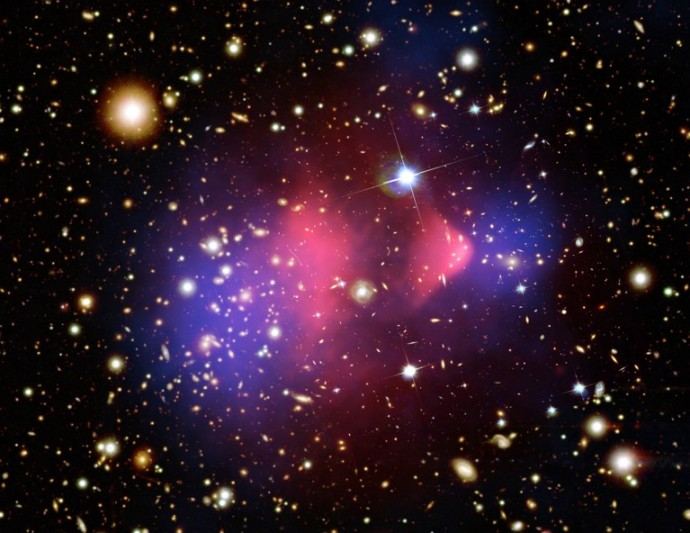
\includegraphics[width=\linewidth]{bullet_cluster}\\
    \tiny{(Clowe et al., \emph{ApJL} 2006)}
  \end{textblock}	
  
  \vspace{8mm}
  The only way to consistently explain:
  \begin{enumerate}
  \item
    rotation curves + vel.~dispersions
  \item
    gravitational lensing
  \item
    cosmological data
	\begin{itemize}  	
	\item    
		Large-scale structure (2dF/Chandra/SDSS-BAO) says $\Omega_\mathrm{matter}\approx 0.27$ 
	\item
		BBN says that $\Omega_\mathrm{baryonic} \approx 0.04$
        \item
                $\implies \Omega_\mathrm{non-baryonic} \approx 5 \times \Omega_\mathrm{baryons}$
        \item
                CMB (WMAP) and SN1a agree; also indicate that $\Omega_\mathrm{total}\approx 1$ 
	\item
		$\implies$ universe is 23\% dark matter, 4\% baryonic (visible) matter, 73\% something else
	\end{itemize}
  \end{enumerate}
\end{frame}

\subsection{Models and requirements}

\begin{frame}
  \frametitle{What we know about it}
  \begin{columns}[T]
	\column{0.1\textwidth}
	
\includegraphics[width=\linewidth]{DM}
	\column{0.95\textwidth}	
	\alert<1-2>{Must be:}
        \begin{itemize}
        \footnotesize
	\item massive (gravitationally-interacting)
        \item unable to interact via the electromagnetic force (dark)
        \item non-baryonic
        \item ``cold(ish)'' (in order to allow structure formation) 
        \item stable on cosmological timescales
        \item produced with the right relic abundance in the early Universe.\\\vspace{2mm}
	\end{itemize}
        \alert<1-2>{Good options:}
        \begin{itemize}
        \footnotesize
        \item \alert<3>{Weakly Interacting Massive Particles (WIMPs)}
        \item sterile neutrinos
        \item gravitinos
        \item axions
        \item axinos
        \item hidden sector dark matter (e.g.~WIMPless dark matter)
        \end{itemize}
  \end{columns}

  \only<2-3>{
  \begin{textblock}{70}(53,63)
    \alert<2>{Bad options:}
    \begin{itemize}
      \footnotesize
      \item primordial black holes% (strong experimental constraints)
      \item MAssive Compact Halo Objects (MACHOs)%; baryonic)
      \item standard model neutrinos %(too warm; insufficient relic density)
    \end{itemize}
  \end{textblock}}

\end{frame}


\begin{frame}
  \frametitle{WIMPs at a glance}
  
  \begin{itemize}
    \item
    Dark because no electromagnetic interactions
    \item
    Cold because very massive ($\sim$10 GeV to $\sim$10 TeV)
    \item
    Non-baryonic and stable - no problems with BBN or CMB
    \item
    Weak-scale annihilation cross-sections \emph{naturally} lead to a relic abundance of the right order of magnitude (more later)
    \item
    Simplest example is scalar singlet dark matter: $\mathcal{L}_S = -\frac{\mu_S^2}{2}S^2 - \frac{\lambda_{hs}}{2}S^2H^\dagger H + \ldots$ 
  \end{itemize}

  \vspace{4cm}

  \begin{textblock}{47}(62,43)
  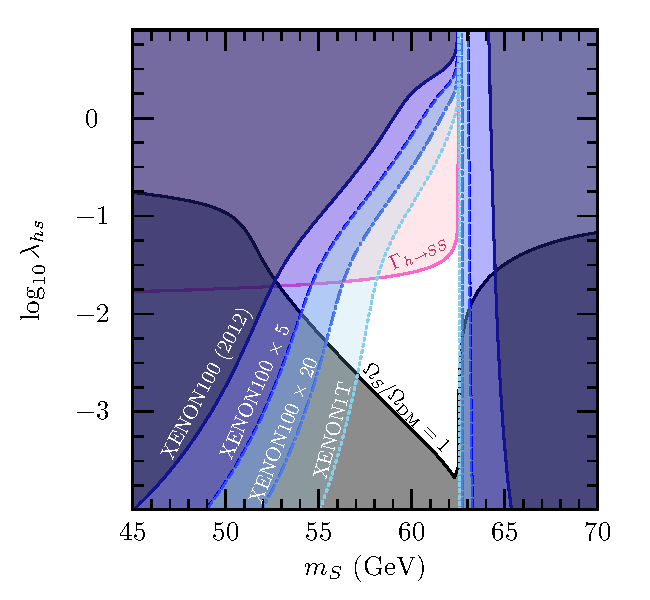
\includegraphics[width=\linewidth]{Fig6a}
  \end{textblock}

  \begin{textblock}{50}(5,76)
    \tiny Cline, Kainulainen, PS \& Weniger \emph{Phys Rev D} 2013
  \end{textblock}


\end{frame}


\begin{frame}
  \frametitle{WIMPs at a glance}
  
  \begin{itemize}
    \item
    Many theoretically well-motivated particle candidates 
      \begin{itemize}
        \footnotesize
        \item
          Supersymmetric (SUSY) neutralinos $\chi$ if $R$-parity is conserved - lightest mixture of neutral higgsinos and gauginos	
	\item
	  Inert Higgses - extra Higgs in the Standard Model
	\item
	  Kaluza-Klein particles - extra dimensions
	\item
 	  right-handed neutrinos, sneutrinos, other exotic things\ldots	  
       \end{itemize}
    \item
    Weak interaction means scattering with nuclei \\$\implies$ detection channel
    \item
    Many WIMPs are Majorana particles (own antiparticles) $\implies$ self-annihilation cross-section

  \end{itemize}

  \centering
  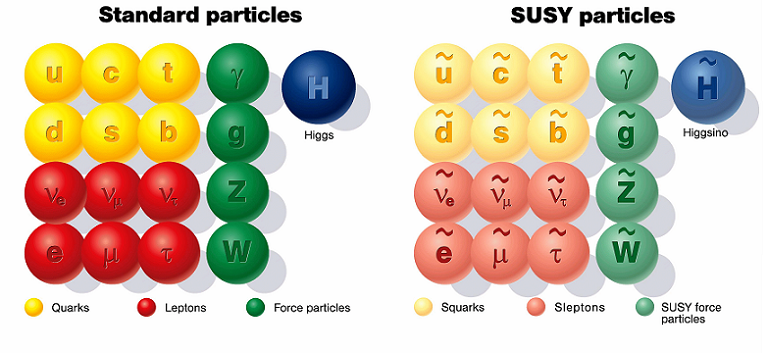
\includegraphics[width=0.64\linewidth]{susyparticles}

\end{frame}


\begin{frame}
  \frametitle{Ways to detect WIMPs}
  \begin{itemize}
  \alert<2>{
    \item Direct detection -- nuclear collisions and recoils
    \item Indirect detection -- annihilations producing SM particles
    \item Impacts on stars -- the Sun and ``dark stars''
  }
  \item Direct production -- missing $E_\mathrm{T}$ or otherwise -- LHC, Tevatron
  \end{itemize}
\end{frame}


\section{Production of dark matter}

\bfr{Thermal and non-thermal production}

\textbf{Thermal Production}\\
\footnotesize
Everything is in perfect thermal equilibrium in early Universe
  \begin{itemize}
    \item[$\implies$] \bi \footnotesize \item Particle populations are all in equilibrium (cf Saha, Boltzmann Eqs) \alert{$\rightarrow$ set by $T$} 
                                        \item Velocities are all in kinetic equilibrium (cf Maxwell dist) \\\alert{$\rightarrow$ set by $T$} \ei  
    \item[$\implies$] As stuff falls out of equilibrium, populations and velocities must be evolved explicitly
    \item[$\implies$] Always present at some level, not always dominant in $\Omega_\mathrm{DM}$
  \end{itemize}\vspace{3mm}

\normalsize
\textbf{Non-thermal Production}\\
\footnotesize
Any other process that dominates the DM relic density\bi
\item Some other heavy BSM particle $X$ decays $\rightarrow$ DM
\item Decays/evaporations of topological defects like cosmic strings
\item Evaporation of PBHs
\item Not always present
\ei

\end{frame}

\bfr{Thermal production}
Thermal relic particle populations (=relic density) are obtained by solving the Boltzmann Equation:
\begin{equation}
\frac{\mathrm{d}n_\chi}{\mathrm{d}t} + 3Hn_\chi = \langle\sigma v\rangle (n_{\chi,\,\mathrm{eq}}^{\phantom{\chi,\,\mathrm{eq}}2} - n_\chi^{\phantom\chi2})
\label{boltzmann}
\end{equation}

\begin{textblock}{50}(70,10)
  \tiny{\color[rgb]{1,1,1}(Kolb \& Turner 1990) $\rightarrow$ DarkSUSY, MicrOmegas, MadDM, SuperIsoRelic, BYO homebrew, etc} 
\end{textblock}

\centering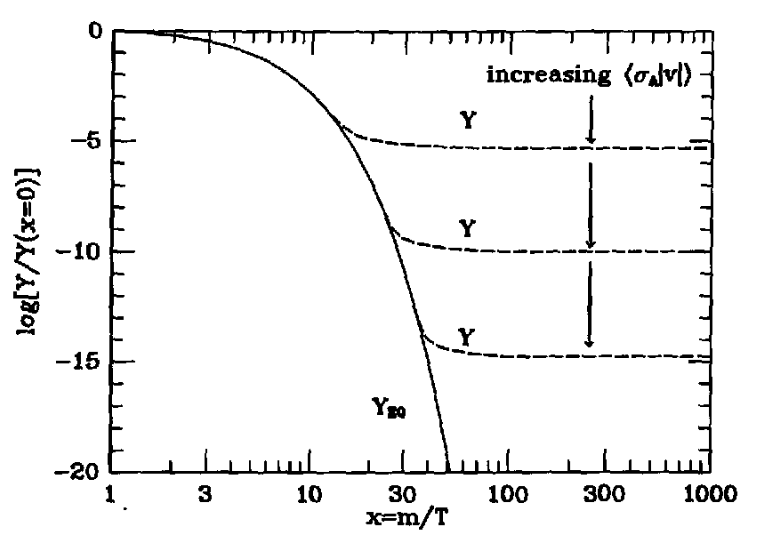
\includegraphics[width=0.55\linewidth]{FreezeOut_KolbTurner}

\end{frame}


\bfr{Kinetic decoupling and small-scale structure}

\footnotesize
\begin{columns}
\column{0.7\textwidth}
\bi
\item Particle production and abundance is \alert{chemical freeze-out}
\item Particle velocities and final DM temperature are determined by \alert{kinetic freeze-out}
\item Typically happen kind of around the same time, but very model-dependent
\item Kinetic decoupling temperature $\rightarrow$ kinetic decoupling scale $\rightarrow$ minimum DM halo mass
\item Impacts boost factors for indirect detection ($\Phi\varpropto\rho^2$), minihalo searches
\ei
\column{0.45\textwidth}
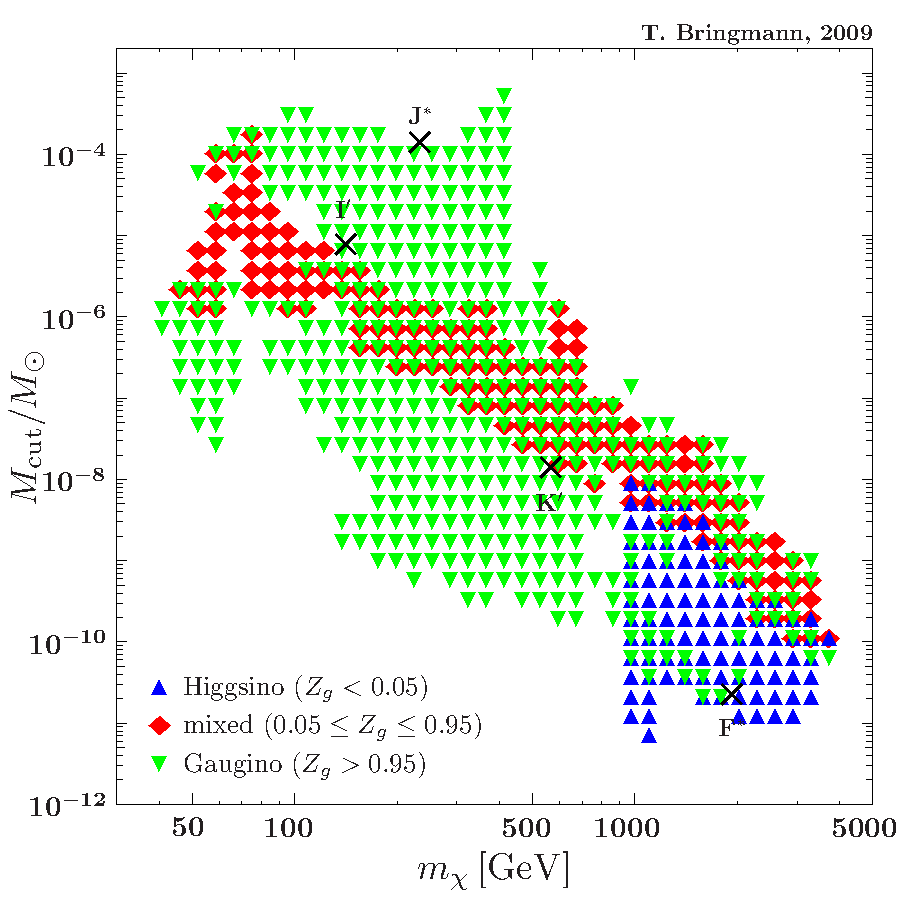
\includegraphics[width=\linewidth]{Mcut}
\end{columns}

\end{frame}


\bfr{Kinetic decoupling and small-scale structure}

Reminder from last lecture: Validity of UCMH limits depend a bit on kinetic decoupling scale
  \vspace{-20mm}
  \begin{columns}
  \column{\textwidth}
    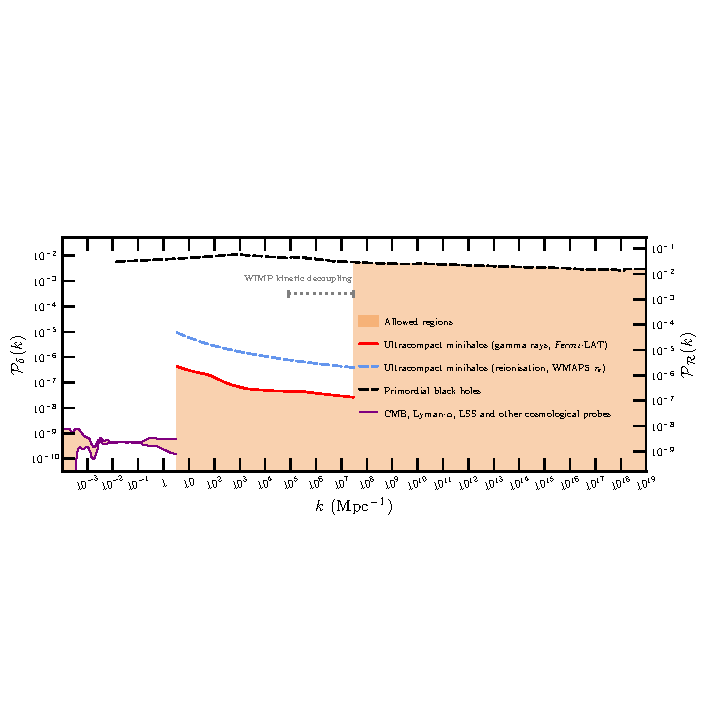
\includegraphics[width=\columnwidth]{Fig6}
  \end{columns}

\end{frame}


\section{Detection of dark matter}

\subsection{Indirect detection}

  \begin{frame}
    \frametitle{Outline of Lecture 2}
  \begin{columns}[t]
	\column{0.8\textwidth}
	\tableofcontents[sections={1},currentsection,currentsubsection]
        \vspace{3mm}
	\tableofcontents[sections={2},currentsection,currentsubsection]
        \vspace{3mm}
	\tableofcontents[sections={3},currentsection,currentsubsection]
  \end{columns}	
  \end{frame}

\bfr{What is indirect detection?}
Looking for Standard Model particles produced by dark matter annihilation or decay: 
  \begin{itemize}
    \footnotesize
    \item{gamma-rays -- \alert<2>{\emph{Fermi}}, HESS, \alert<2>{CTA}}
    \item{anti-protons -- PAMELA, AMS-02}
    \item{anti-deuterons -- GAPS}
    \item{neutrinos -- \alert<2>{IceCube}, ANTARES}
    \item{$e^+e^-$ -- \alert<2>{PAMELA}, \emph{Fermi}, ATIC, \alert<2>{AMS-02}}\\
    {$\rightarrow$ secondary radiation: inverse Compton, synchrotron, bremsstrahlung}
    \item{\alert<2>{secondary impacts on the CMB}, reionisation}
  \end{itemize}

\end{frame}


\begin{frame}
  \frametitle{Finding dark matter with neutrino telescopes}

\begin{columns}[c]
\column{0.75\textwidth}
The cartoon version: \begin{enumerate}
\item \visible<2->{Halo WIMPs crash into the Sun}
\item \visible<3->{Some lose enough energy in the scatter to be gravitationally bound}
\item \visible<4->{Scatter some more, sink to the core}
\item \visible<5->{Annihilate with each other, producing neutrinos}
\item \visible<6->{Propagate+oscillate their way to the Earth, convert into muons in ice/water}
\item \visible<7->{Look for \v{C}erenkov radiation from the muons in \textbf{IceCube}, ANTARES, etc}
\end{enumerate}
\column{0.35\textwidth}
  \visible<2->{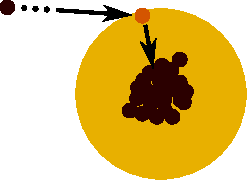
\includegraphics[width=0.8\columnwidth]{comic3_1}}\\
  \visible<4->{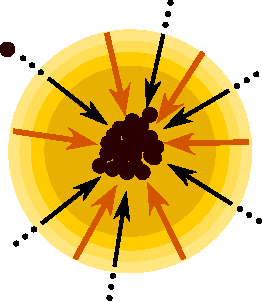
\includegraphics[width=0.6\columnwidth]{comic3_2}}\\
  \visible<5->{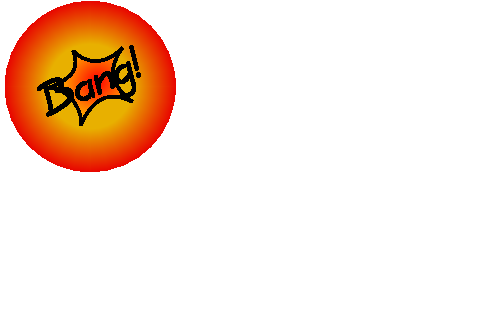
\includegraphics[width=0.6\columnwidth, trim = 0 70 150 0, clip=true]{comic_4}}
\end{columns}

\end{frame}

\begin{frame}
\frametitle{The IceCube Neutrino Observatory}

\begin{columns}[c]
\column{0.4\linewidth}
\begin{itemize}
\item 86 strings
\item 1.5--2.5\,km deep in Antarctic ice sheet
\item $\sim$125\,m spacing between strings
\item $\sim$70\,m in DeepCore (10$\times$ higher optical detector density)
\item 1\,km$^3$ instrumented volume (1\,Gton)
\end{itemize}
\column{0.6\linewidth}
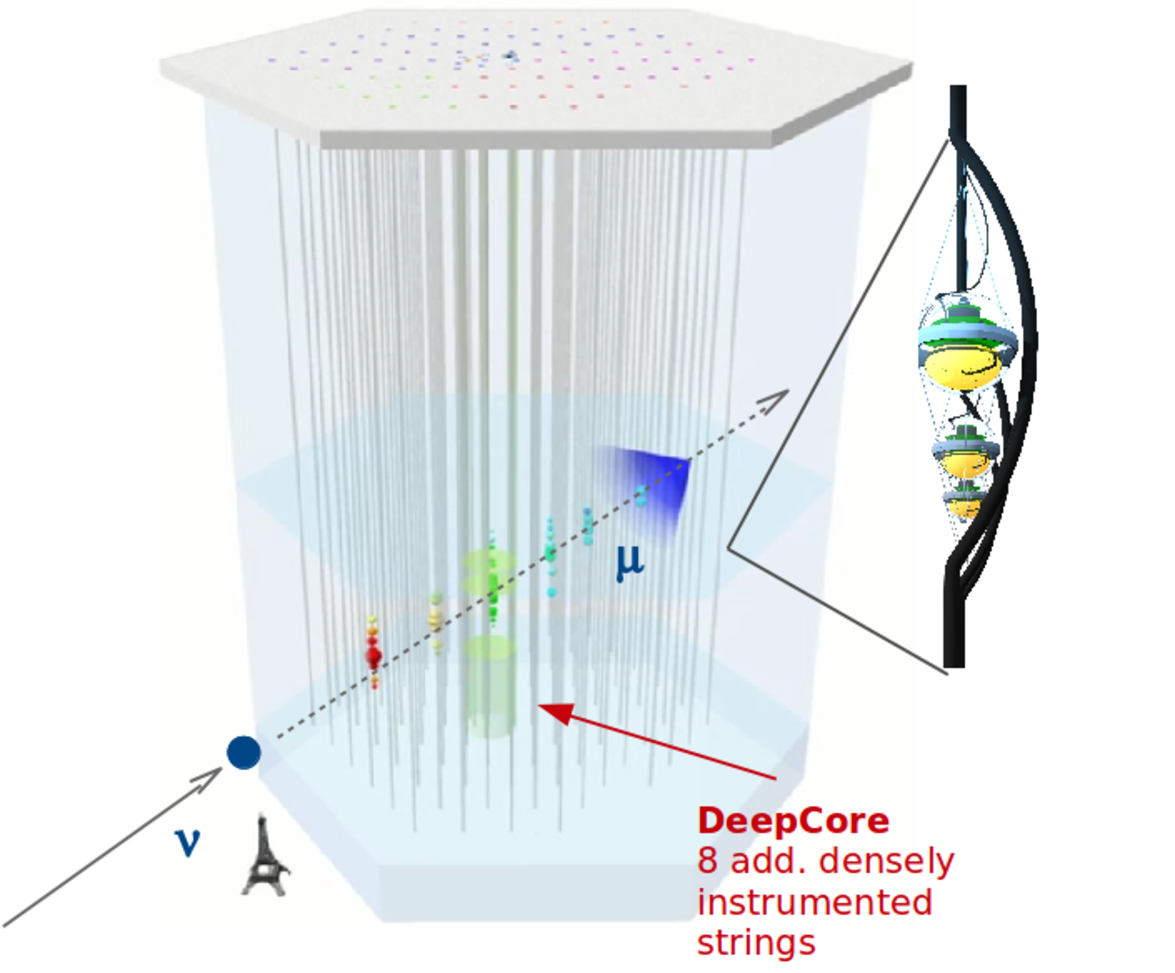
\includegraphics[width=\columnwidth]{icecube}
\end{columns}
\end{frame}


\begin{frame}
\frametitle{Neutrino limits from IceCube}

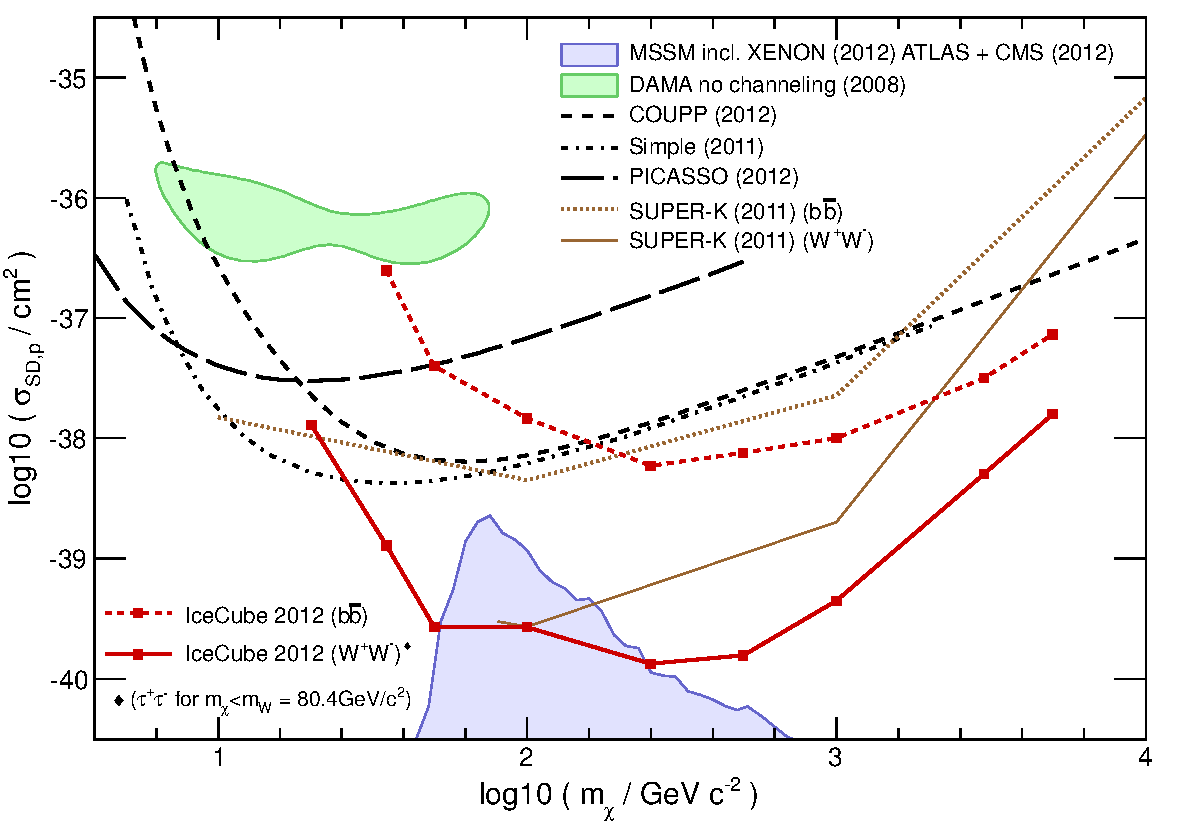
\includegraphics[width=0.8\columnwidth]{fig3}

\tiny IceCube Collaboration, \emph{Phys.\ Rev.\ Lett.} 2013\\
      Theory region: MSSM-25 from Silverwood, PS, Danninger, et al \emph{JCAP} 2012

\end{frame}

\begin{frame}
  \frametitle{Gamma-rays from dark matter}
  \begin{columns}[c]
    \column{0.32\textwidth}
      \centering
      \visible<2-4>{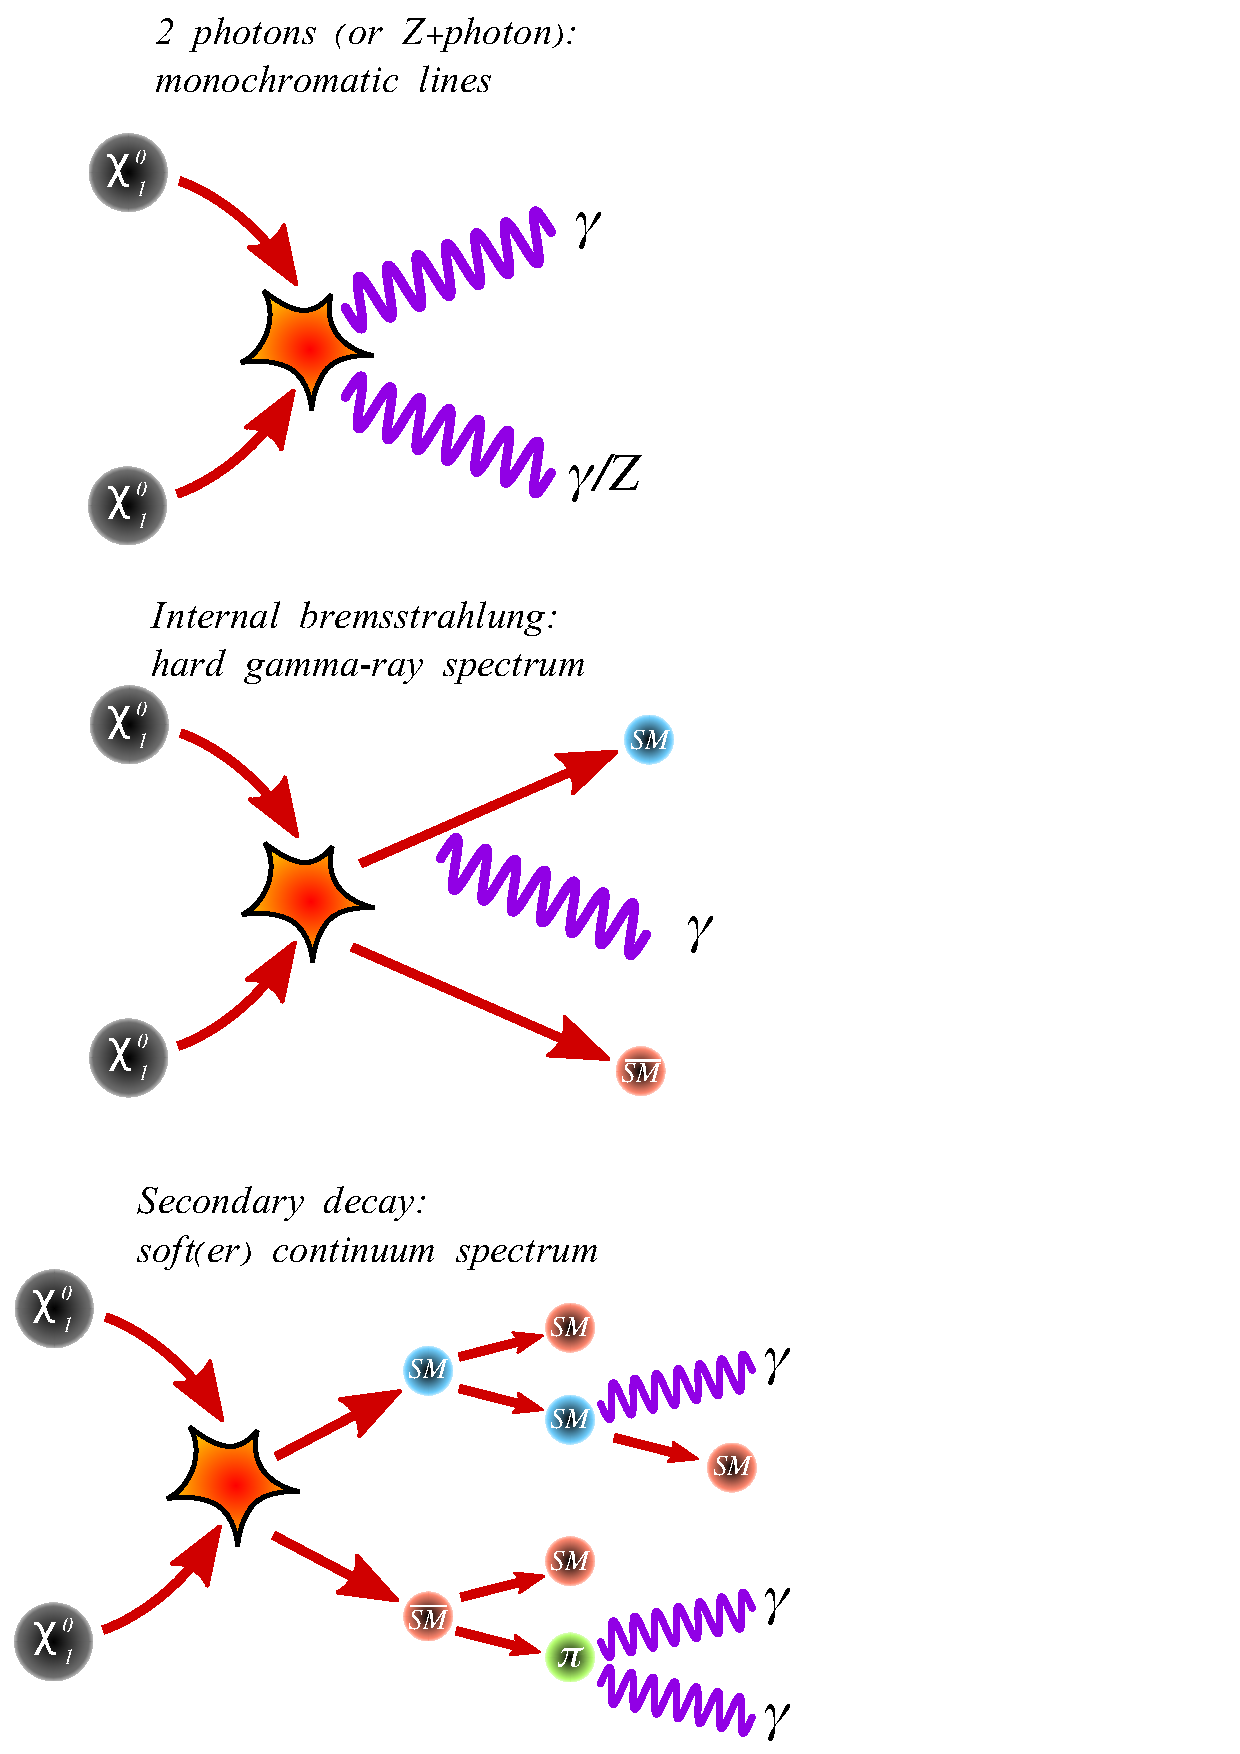
\includegraphics[width=\columnwidth, trim = 0 560 240 0, clip=true]{chi_annihilation}}\\
    \column{0.32\textwidth}
      \centering
      \visible<3-4>{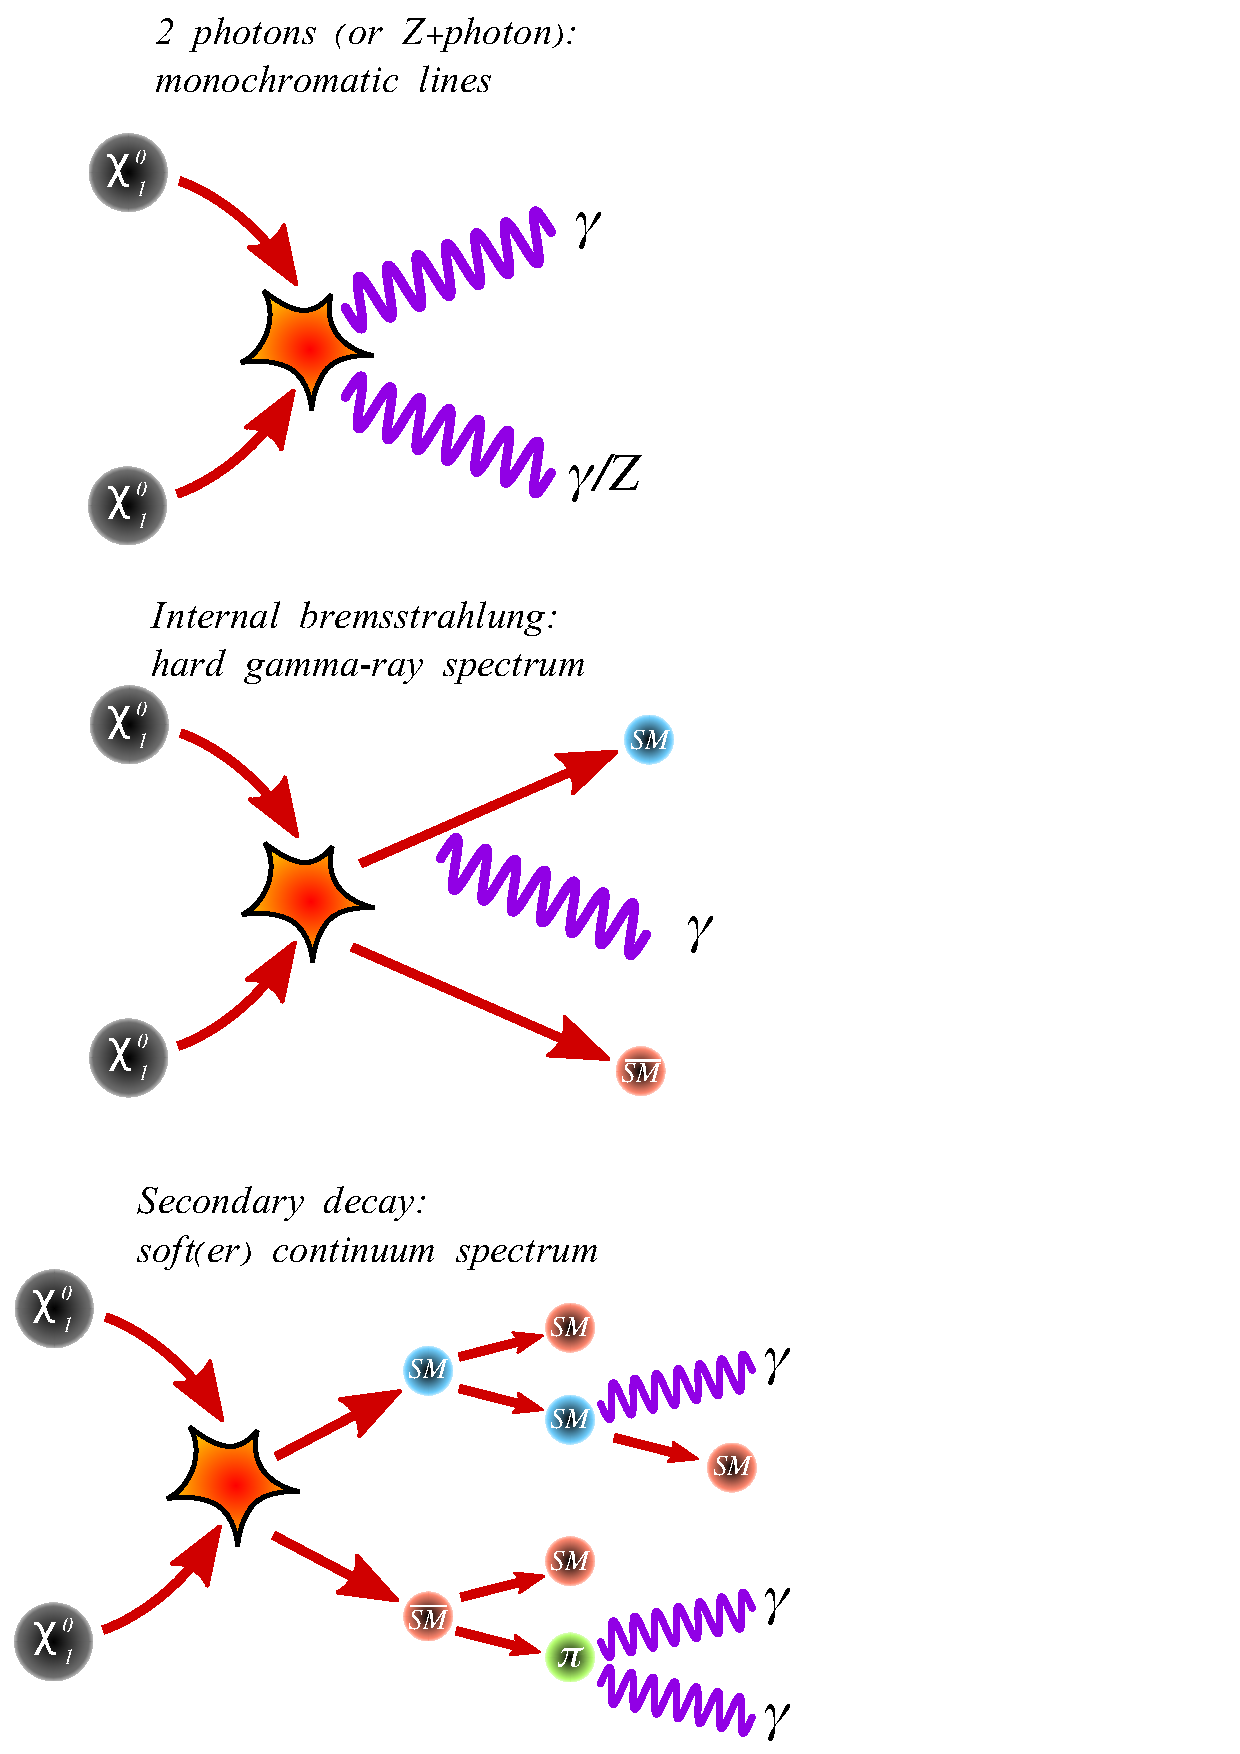
\includegraphics[width=\columnwidth, trim = 0 280 240 280, clip=true]{chi_annihilation}}\\
    \column{0.36\textwidth}
      \centering
      \visible<4>{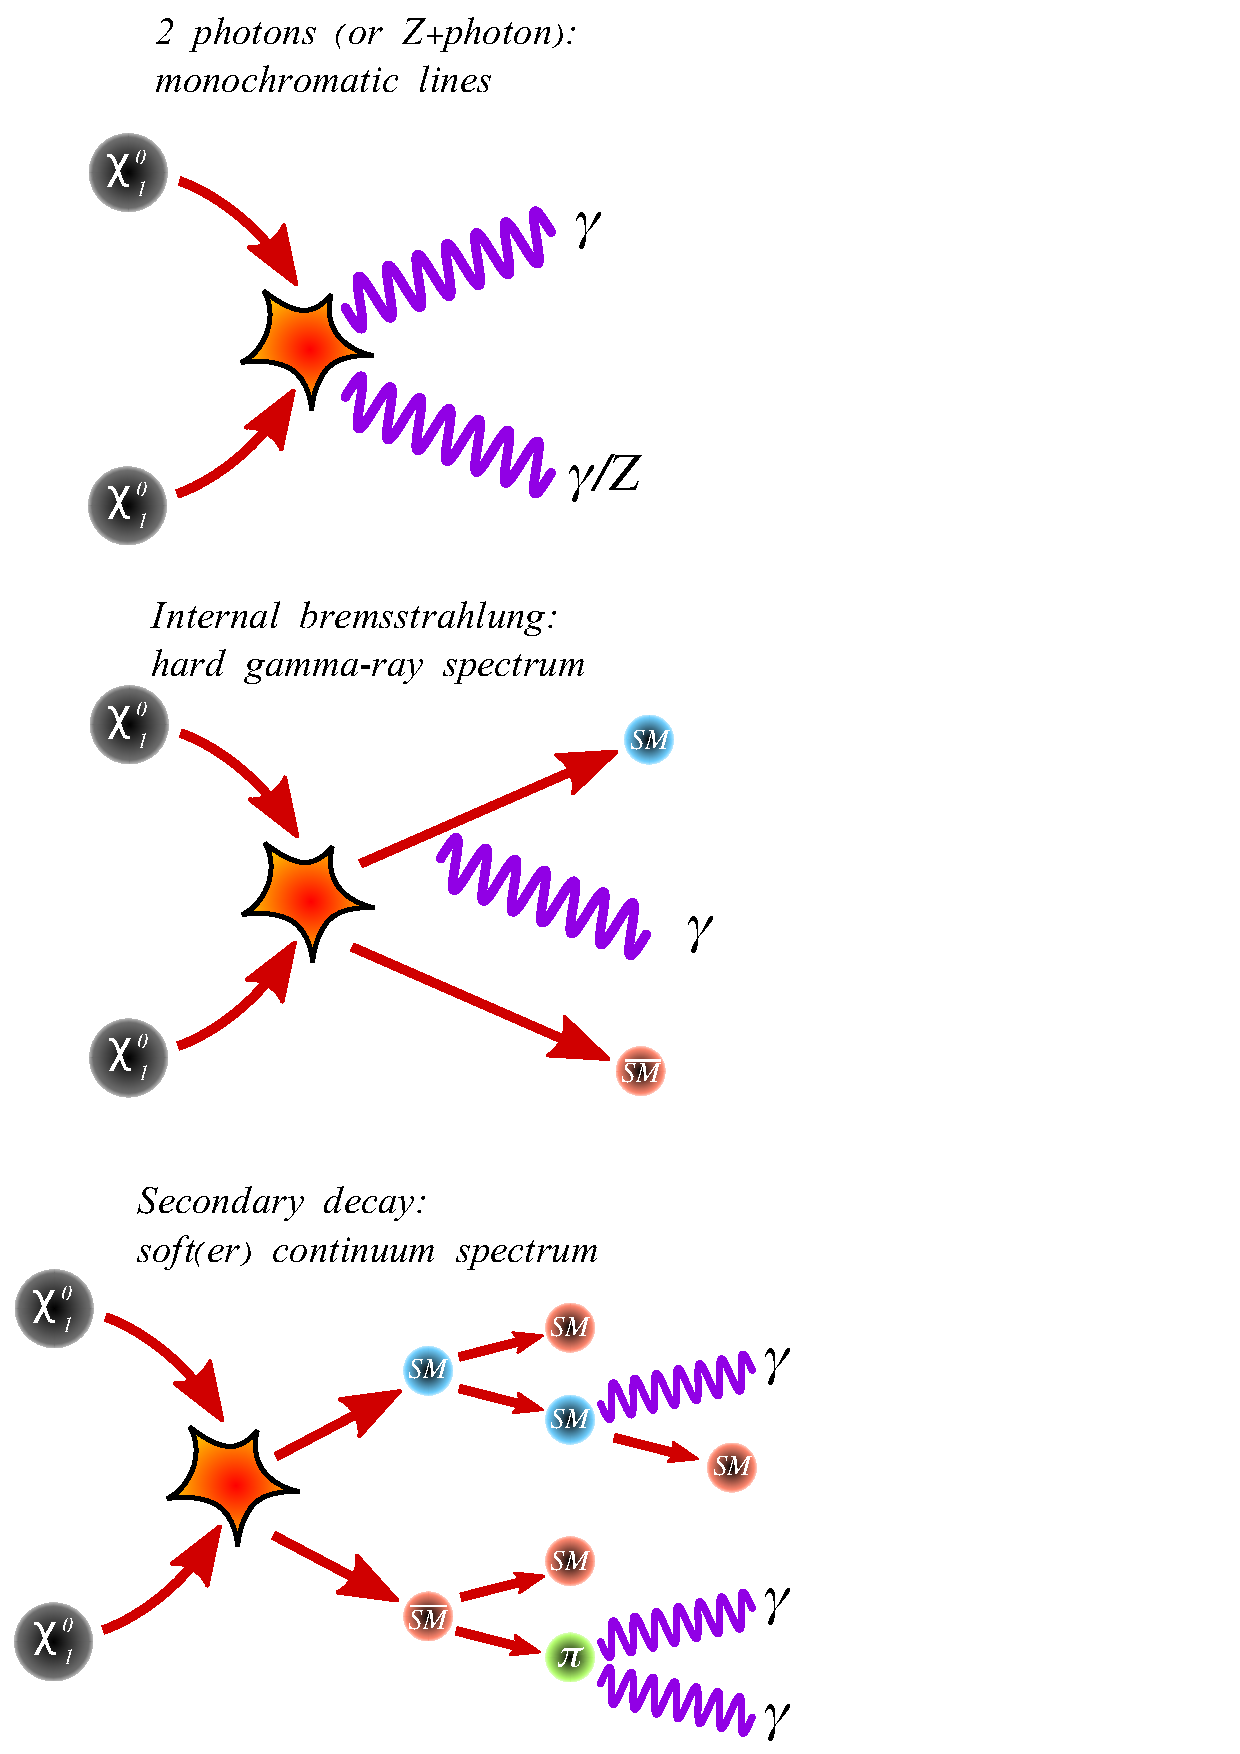
\includegraphics[width=\columnwidth, trim = 0 0 210 560, clip=true]{chi_annihilation}}\\
    \end{columns}

      \begin{itemize}
        \visible<1-4>{\item{3 main gamma-ray channels:
          {\footnotesize\begin{itemize}
          \visible<2-4>{\item monochromatic lines}
          \visible<3-4>{\item internal bremsstrahlung (FSR + VIB)}
          \visible<4>{\item continuum from secondary decay}
          \end{itemize}}}}
      \end{itemize}
\end{frame}

\begin{frame}
  \frametitle{Targets}

  \vspace{-9mm}
  \begin{itemize}
    \item{$\Phi \varpropto$ annihilation~rate $\varpropto \rho_\mathrm{DM}^2$}
  \end{itemize}
  Likely targets:
    \begin{itemize}

      \uncover<2-9>{\item \alert<7-9>{Galactic centre} - large signal, large BG}
      \visible<1-6,10-11>{\uncover<3-6>{\item Galactic halo - moderate signal, moderate BG}
      \uncover<4-6,10>{\item \alert<9>{dwarf galaxies} - low statistics, low BG}}
      \visible<1-6,11>{\uncover<5-6>{\item clusters/extragalactic diffuse - large modelling uncertainties, low signal, low BG}
      \uncover<6,11>{\item \alert<10>{dark clumps} - low statistics, low BG}}
      
    \end{itemize}

\begin{textblock}{105}(40,20)
\only<10>{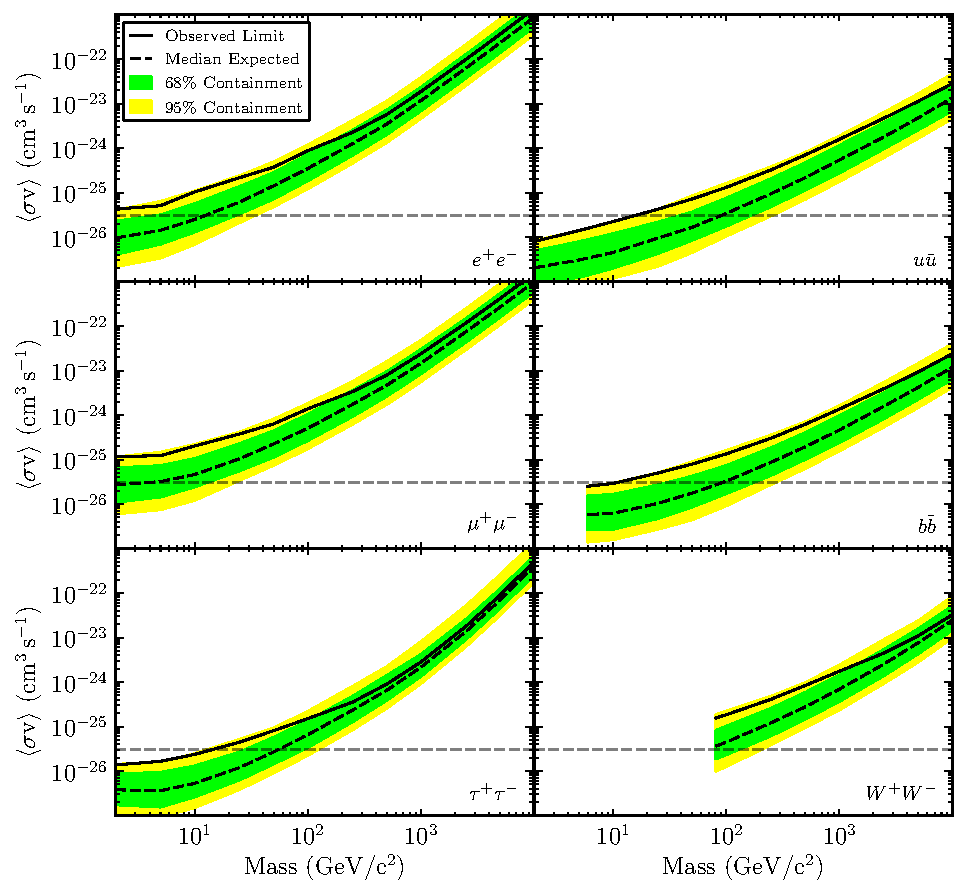
\includegraphics[width=0.7\columnwidth, trim = 0 0 0 0, clip=true]{composite_limit_data_plot}}
\end{textblock}

\begin{textblock}{40}(80,10)
\only<10>{\tiny\color[rgb]{1, 1, 1}Fermi-LAT Collab., \emph{Phys. Rev. D} 2014}\color[rgb]{0, 0, 0}
\end{textblock}

\begin{textblock}{105}(4,45)
\only<7>{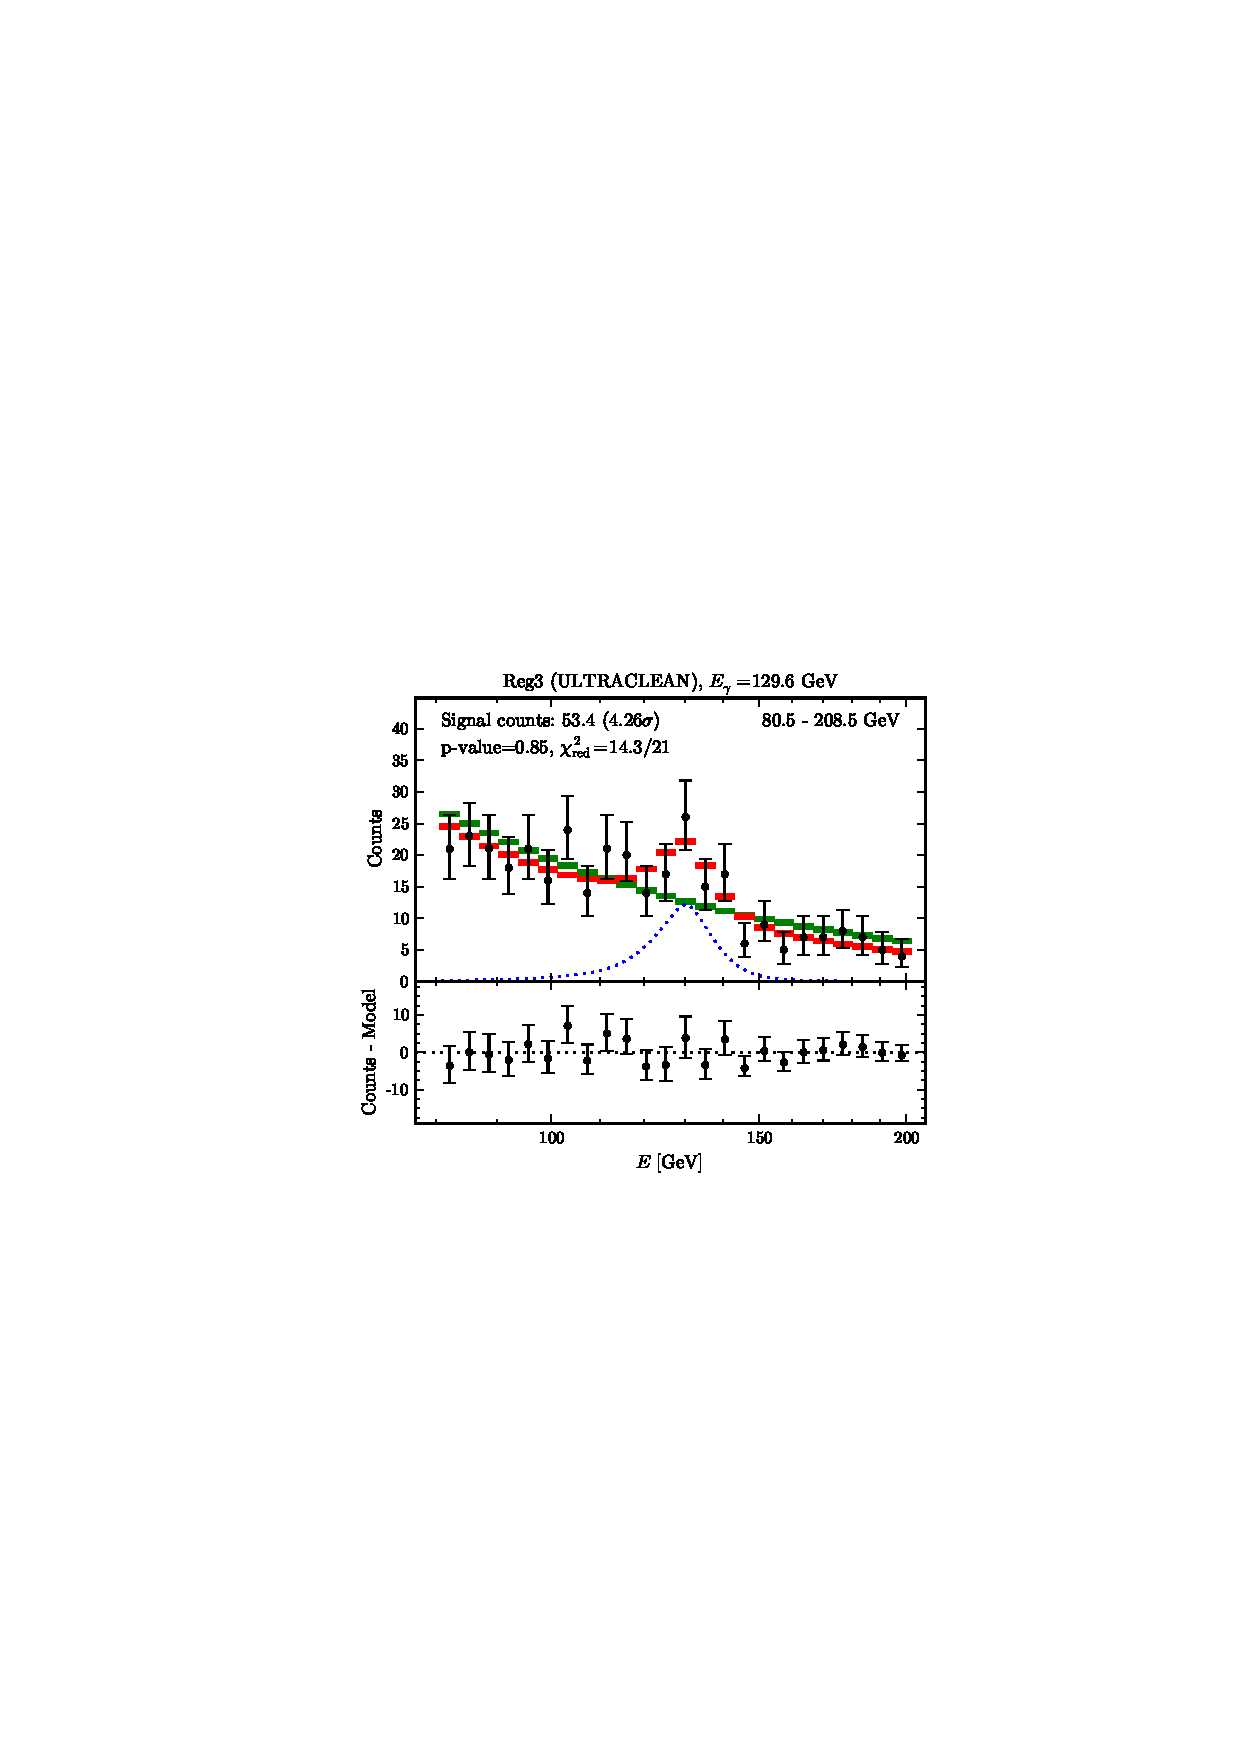
\includegraphics[width=0.44\columnwidth]{line}\hspace{2mm}%
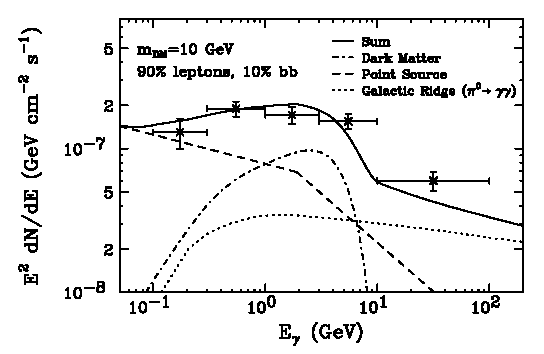
\includegraphics[width=0.54\columnwidth]{Hooper}}
\end{textblock}

\begin{textblock}{105}(4,40)
\only<8>{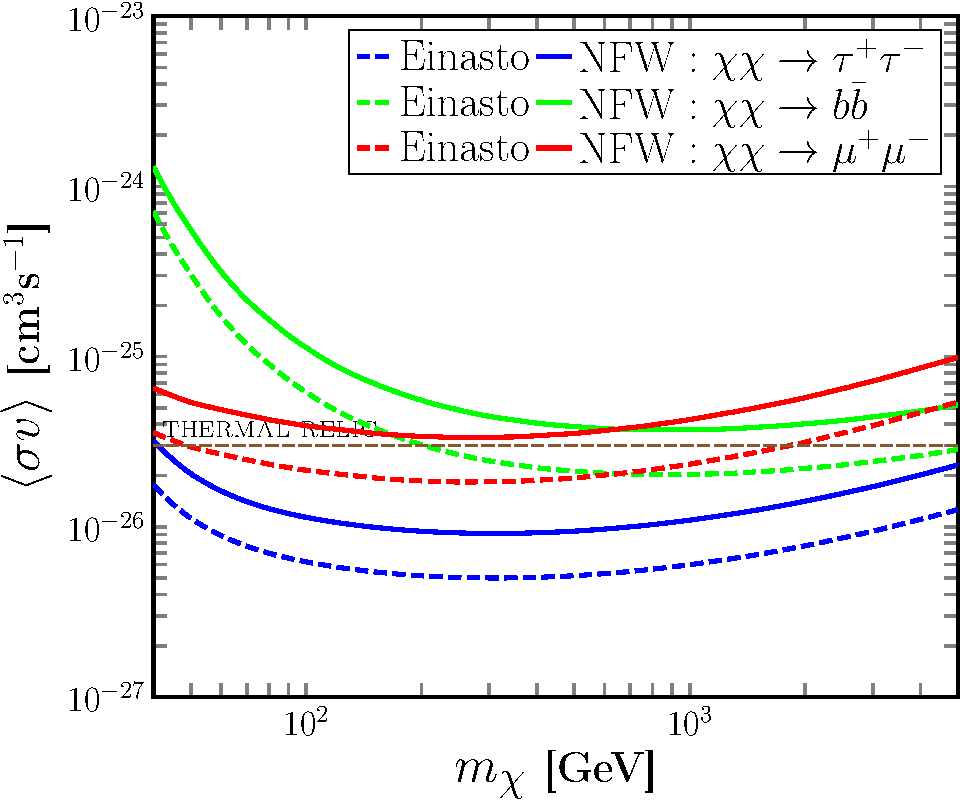
\includegraphics[width=0.49\columnwidth]{CTA1}\hspace{2mm}%
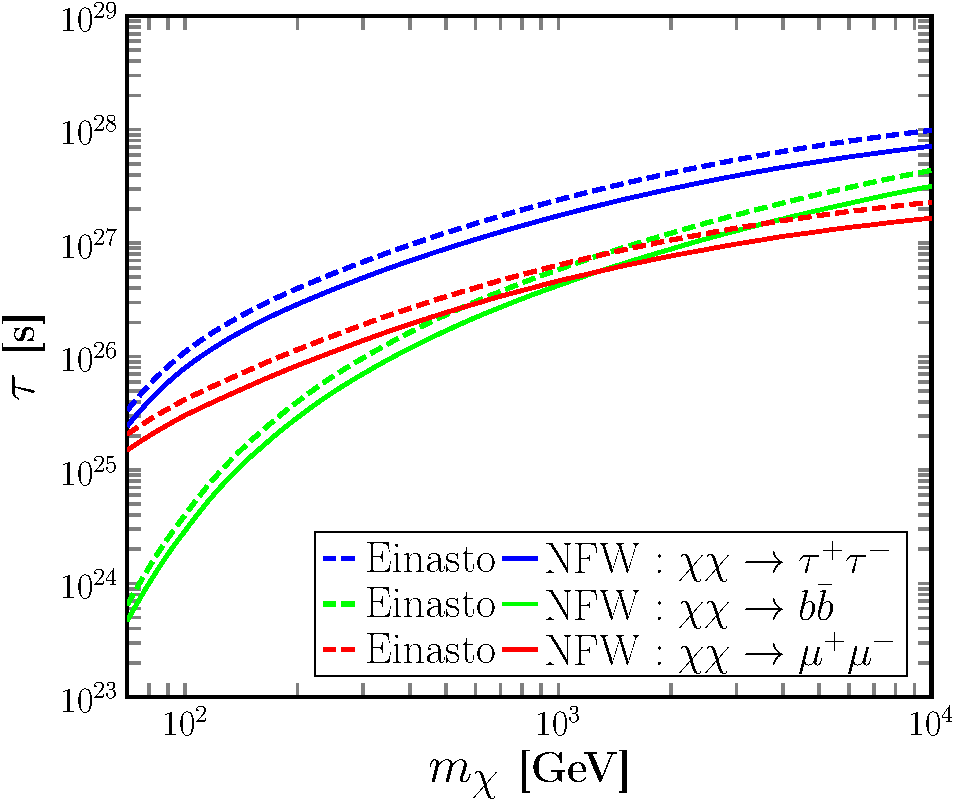
\includegraphics[width=0.49\columnwidth]{CTA2}}
\end{textblock}

\begin{textblock}{105}(4,40)
\only<9>{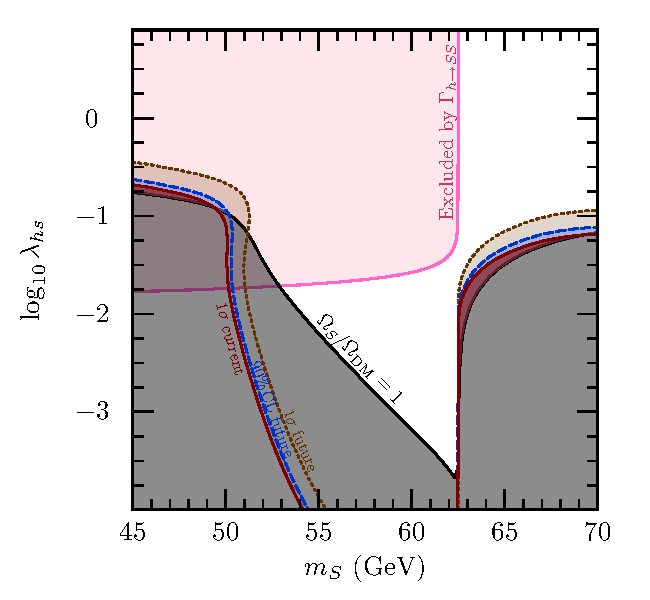
\includegraphics[width=0.49\columnwidth]{Fig3a}\hspace{2mm}%
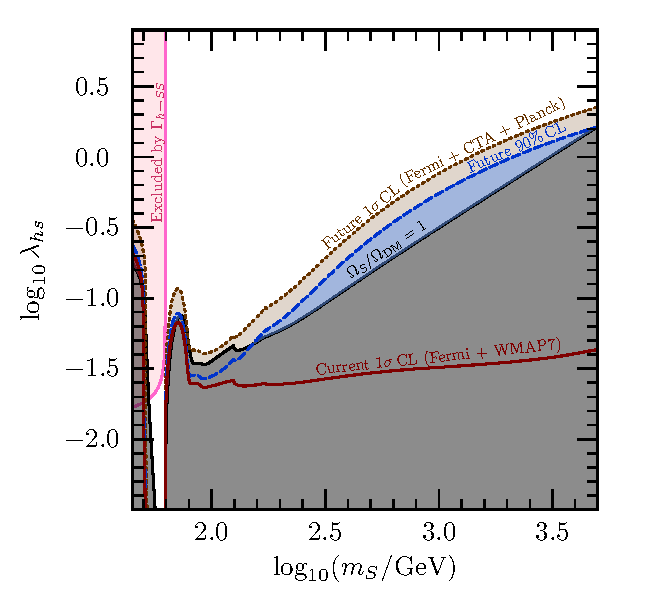
\includegraphics[width=0.49\columnwidth]{Fig3b}}
\end{textblock}

\begin{textblock}{40}(80,10)
\only<7>{\tiny\color[rgb]{1, 1, 1}Weniger,  \emph{JCAP} 2012\\Hooper \& Linden, arXiv:1110.0006}\color[rgb]{0, 0, 0}
\end{textblock}

\begin{textblock}{40}(75,10)
\only<8>{\tiny\color[rgb]{1, 1, 1}Pierre, Siegal-Gaskins \& PS arXiv:1401.7330}\color[rgb]{0, 0, 0}
\end{textblock}

\begin{textblock}{40}(75,10)
\only<9>{\tiny\color[rgb]{1, 1, 1}Cline, Kainulainen, PS \& Weniger \emph{Phys Rev D} 2013}\color[rgb]{0, 0, 0}
\end{textblock}

\end{frame}


\bfr{Impacts of DM annihilation on the CMB}

Energy injection from DM annihilation/decay at $z\sim600$
\bi
\item[$\rightarrow$] Would change ionisation balance via $\gamma$s and $e^+e^-$ interaction with electrons and H
\item[$\rightarrow$] Changes timing + extent of recombination
\item[$\rightarrow$] Distortion of CMB angular power spectrum
\ei
\vspace{4cm}

\begin{textblock}{70}(15,48)
{
    \begin{columns}
    \column{0.6\linewidth}
    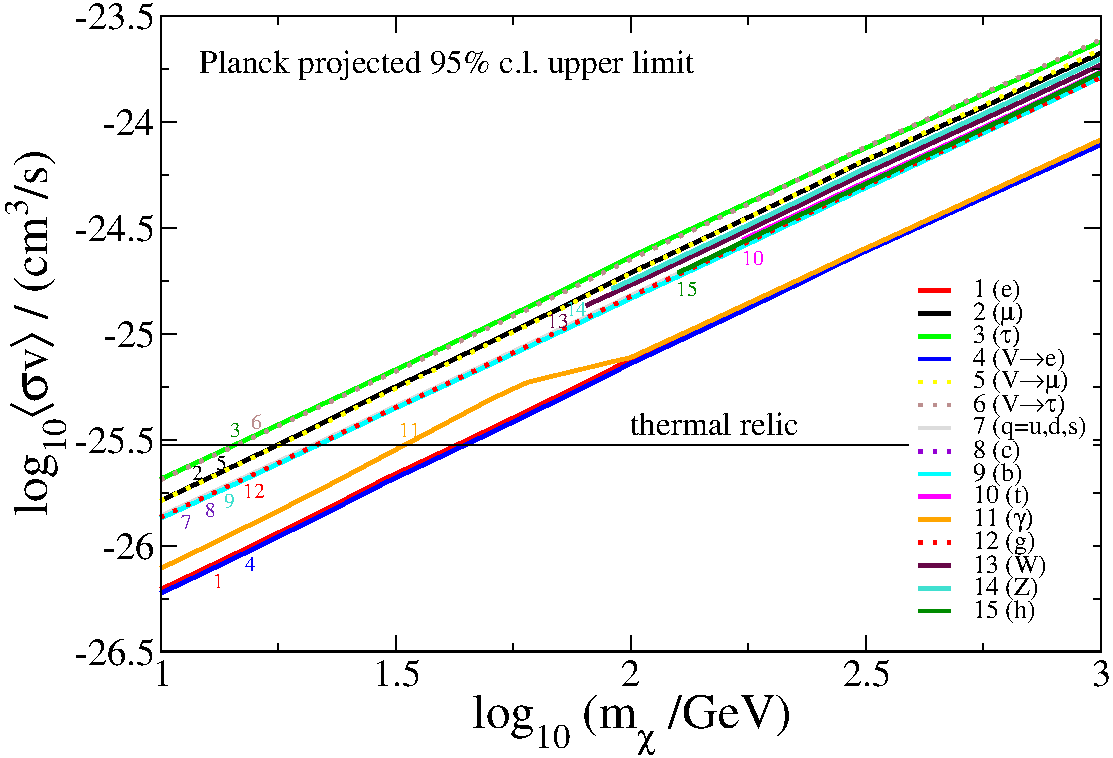
\includegraphics[width=1.1\textwidth]{planck-limit}
    \column{0.1\linewidth}
    \column{0.6\linewidth}
    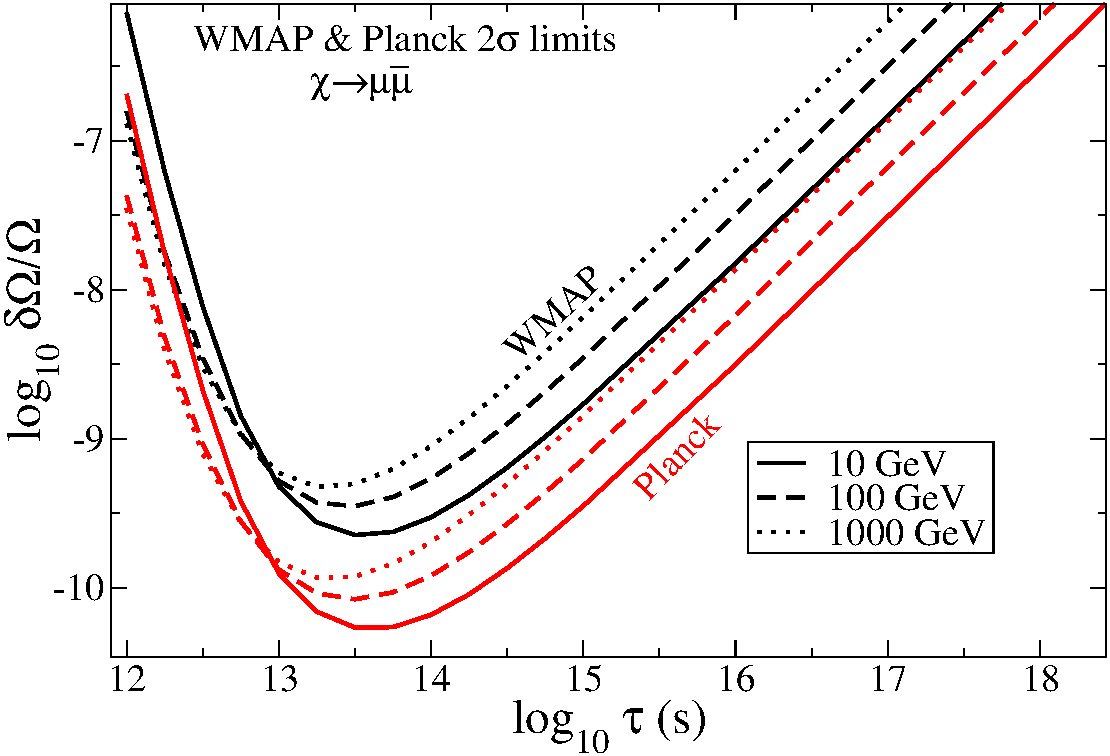
\includegraphics[width=1.1\textwidth]{muons-w-Planck}
    \end{columns}\vspace{1mm}
    \hspace{3cm} \tiny Cline \& PS \textit{JCAP} 2013
}

\end{textblock}


\end{frame}


\bfr{Positrons}

\bi
  \item Excess over expected background (secondary) positron ratio observed
  \item First seen by PAMELA, confirmed by \textit{Fermi} then AMS-02.  Still unexplained.
  \item Could be evidence of dark matter
\ei

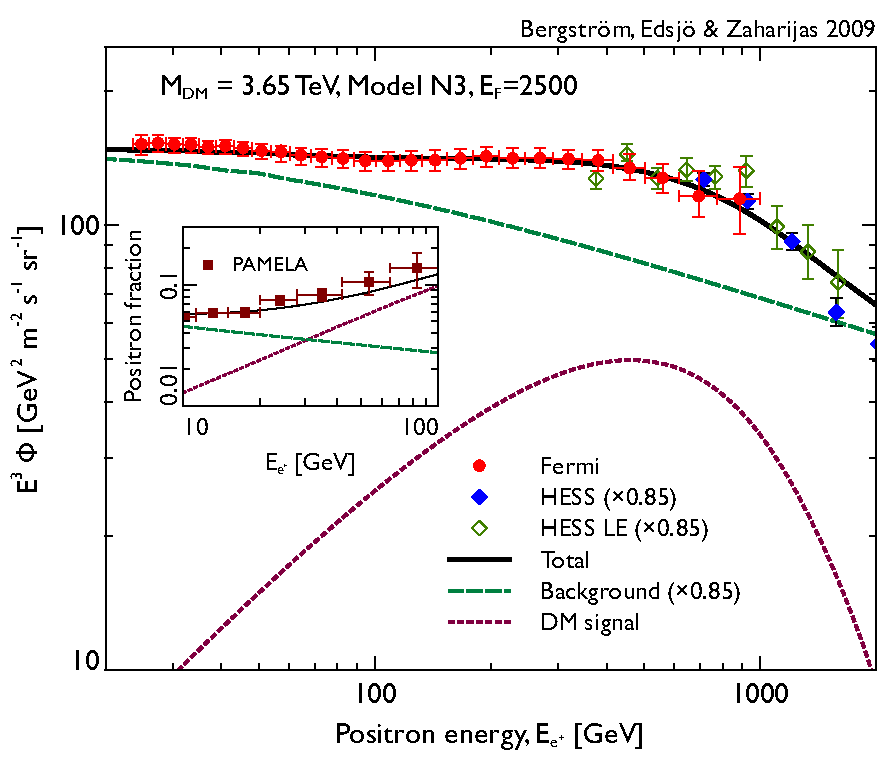
\includegraphics[width=0.45\linewidth]{spec-n3}\hspace{2mm}
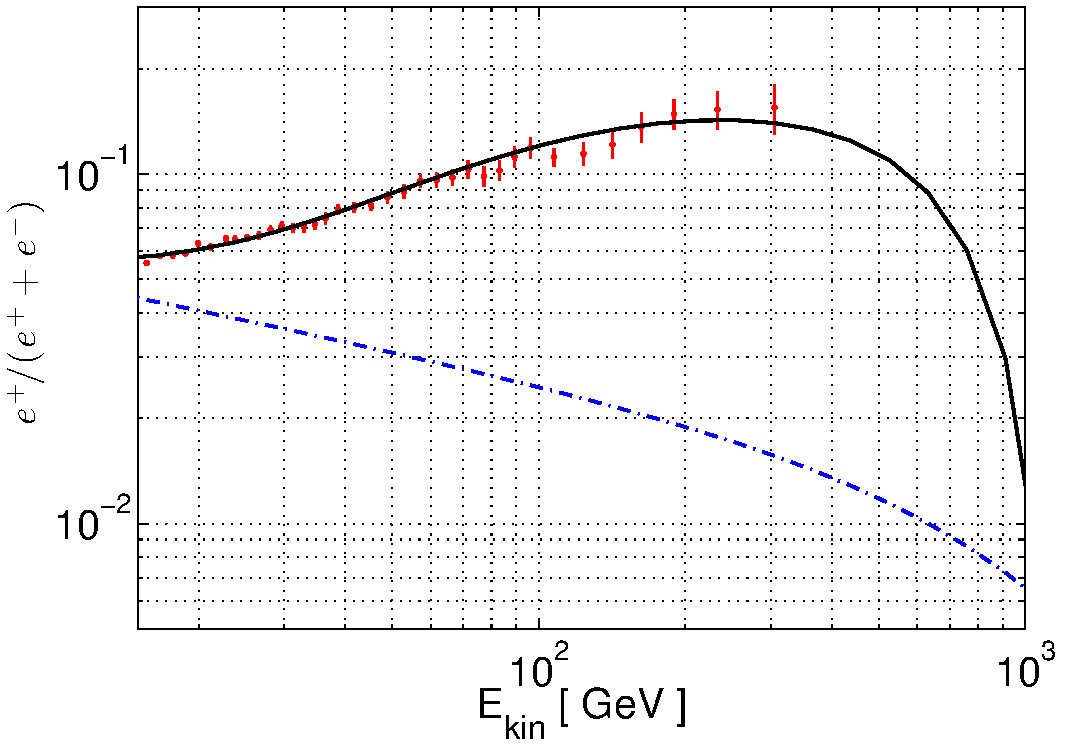
\includegraphics[width=0.51\linewidth]{AMSepr_m2}

\begin{textblock}{35}(73,45)
  {\tiny AMS-02; De Simone et al \textit{JCAP} 2013}
\end{textblock}

\end{frame}



\subsection{Direct detection}

  \begin{frame}
    \frametitle{Outline of Lecture 2}
  \begin{columns}[t]
	\column{0.8\textwidth}
	\tableofcontents[sections={1},currentsection,currentsubsection]
        \vspace{3mm}
	\tableofcontents[sections={2},currentsection,currentsubsection]
        \vspace{3mm}
	\tableofcontents[sections={3},currentsection,currentsubsection]
  \end{columns}	
  \end{frame}

\bfr{Directly detecting dark matter in the lab}

  \begin{itemize}
    \item WIMP flies in, scatters elastically off an atomic nucleus $\implies$ nucleus gets a kick
    \item Very small kick $\implies$ very low threshold detection required
  \end{itemize}
\vspace{1mm}
\begin{displaymath}
\frac{dN}{dE_\mathrm{r}} = \frac{\sigma\rho}{2\mu^2m_{\chi}}F^2\int_{v_\mathrm{min}(E_\mathrm{r})}^{v_\mathrm{esc}}\frac{f(v)}{v}dv
\end{displaymath}

\begin{columns}[T]
\column{0.38\textwidth}
{\tiny
\vspace{1mm}
\begin{tabular}{l@{\,=\,}l}
	$N$ & number of scatterings \\
	$E_\mathrm{r}$ & nuclear recoil energy \\
	$\sigma$ & WIMP-nucleus cross-section \\
	$\rho$ & WIMP density \\
	$\mu$ & WIMP-nucleus reduced mass \\
	$m_\chi$ & WIMP mass \\
	$F$ & nuclear form factor \\
	$f(v)$ & WIMP velocity distribution \\
	$v$ & WIMP velocity \\
	$v_\mathrm{min}(E_\mathrm{r})$ & minimum $v$ to produce recoil $E_\mathrm{r}$ \\  
	$v_\mathrm{esc}$ & halo escape velocity (max $v$) \\ 
\end{tabular}
}
\column{0.62\textwidth}
\vspace{1mm}
Recoil rate is degenerate in unknowns 
\begin{itemize}
	\item
	WIMP mass
	\item
	local WIMP density	
	\item	
	halo velocity distribution
	\item
	WIMP-nucleus cross-section
\end{itemize}
\end{columns}
\end{frame}

\begin{frame}
	\frametitle{Daily \& yearly modulation}
	Due to Earth's proper motion in the galaxy, we expect: 
	\vspace{4mm}

	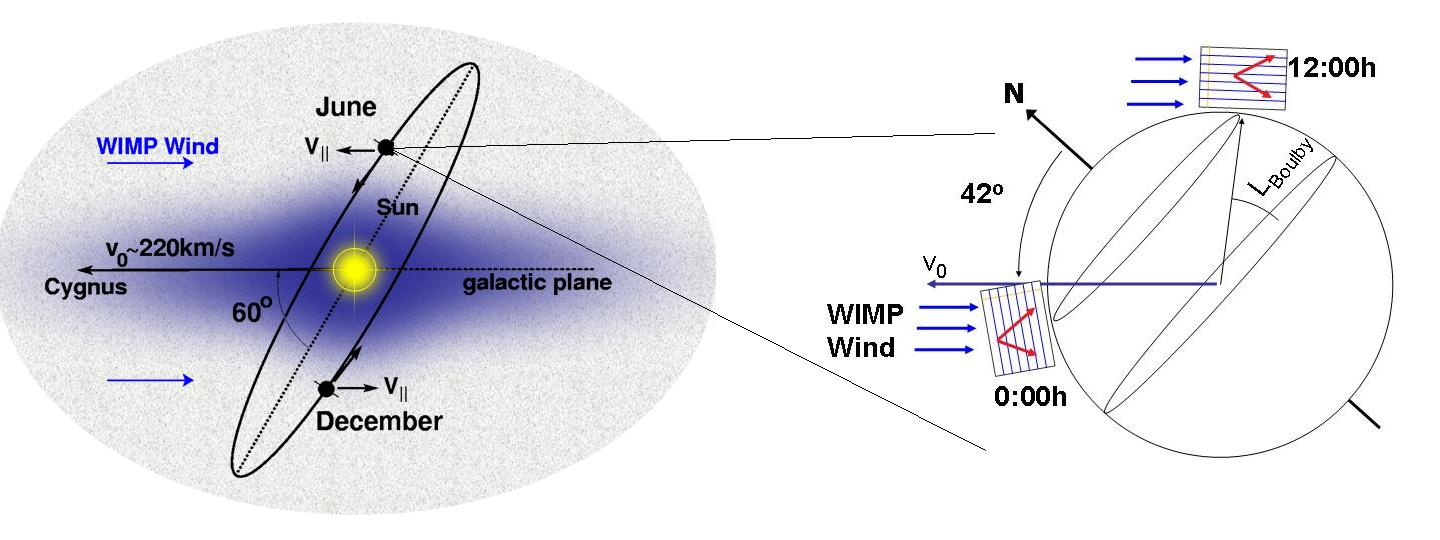
\includegraphics[width=\textwidth]{Modulation}\\
	\vspace{-8mm}
	\begin{columns}[T]
		\column{0.5\textwidth}
		\center{\hspace{8mm}annual modulation}
		\column{0.5\textwidth}
		\center{diurnal (day-night) modulation}
	\end{columns}
\end{frame}

\begin{frame}
	\frametitle{Spin-dependent and -independent cross-sections}
	\begin{columns}[T]
		\column{0.5\textwidth}
		Spin-independent
		\begin{itemize}
		\item
		\alert<2>{Scattering off all nucleons}
		\item
		\alert<3>{$\implies$ proportional to $A^2$ ($A=$ atomic weight)}		
		\item
		\alert<4>{Dominates for heavy nuclei due to $A^2$ enhancement}
		\item
		\alert<4>{Form factor can suppress momentum transfer in very large nuclei though} 
		\item
		\alert<5>{Most studied, most accessible}  		
		\end{itemize}
		\column{0.5\textwidth}
		Spin-dependent
		\begin{itemize}
		\item
		\alert<2>{Scattering only off nucleons with \emph{net} nuclear spin (i.e.~whose spins remain \emph{unpaired})}
		\item
		\alert<3>{$\implies$ less increase with $A$ than spin-independent cross-section}		
		\item
		\alert<4>{Important for light nuclei (e.g. in stars!)}
		\item
		\alert<5>{Least studied, trickier}		
		\end{itemize}
	\end{columns}
\end{frame}

\begin{frame}
	\frametitle{3 ways to detect recoils}
	\begin{columns}[T]
		\column{0.333\textwidth}
		Ionisation\\	
		\vspace{2cm}	
		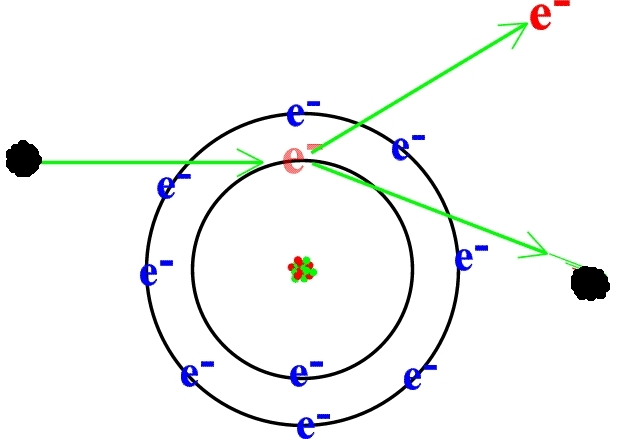
\includegraphics[width=0.8\linewidth]{Ionisation}
		\column{0.333\textwidth}
		Scintillation\\\tiny(just fluorescence with a quick recovery and in a transparent medium)\\
		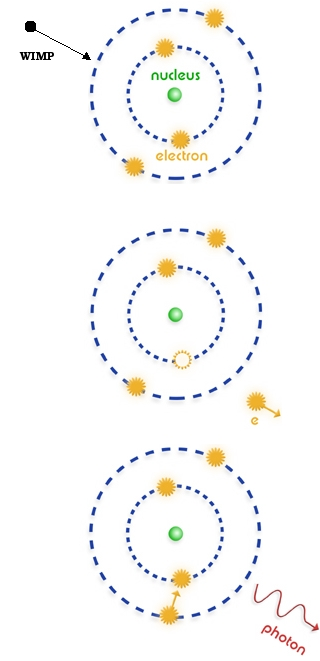
\includegraphics[height=0.7\textheight]{Scintillation}		
		\column{0.333\textwidth}
		Vibration (phonons)\\
		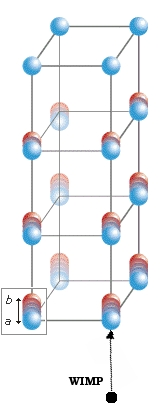
\includegraphics[height=0.7\textheight]{Phonons}
	\end{columns}
  \begin{textblock}{70}(40,40)
    \only<2>{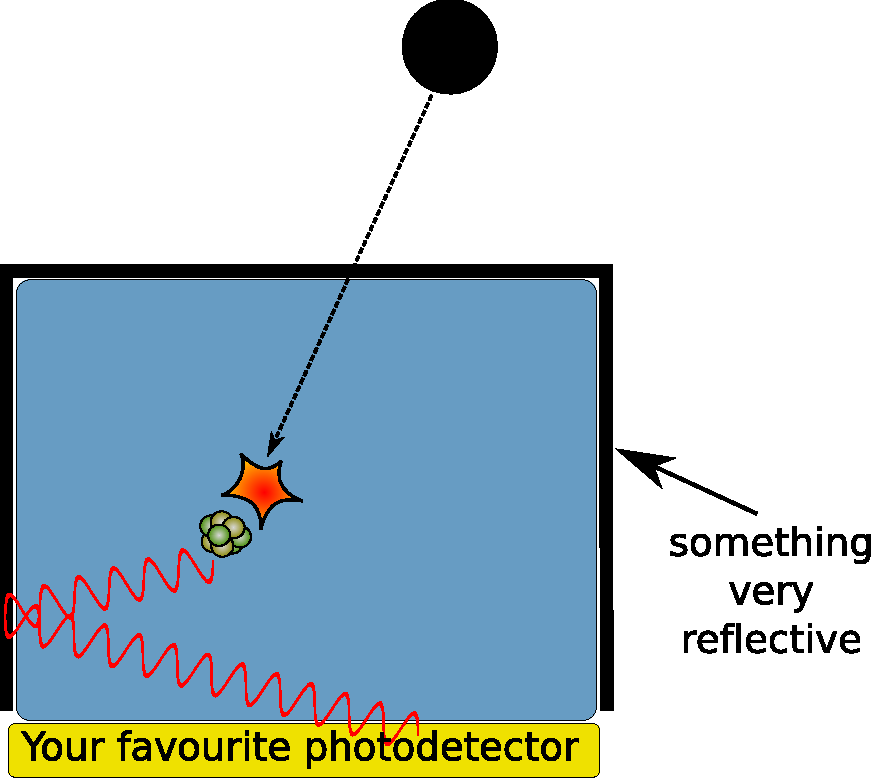
\includegraphics[width=0.6\linewidth]{SolidScintillator}}
  \end{textblock}

  \begin{textblock}{80}(25,40)
    \only<3>{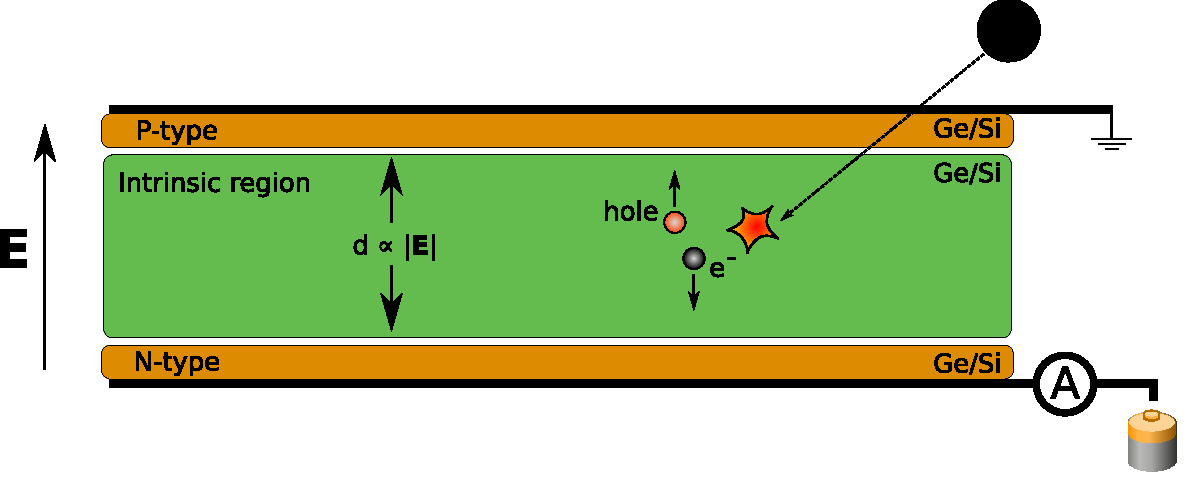
\includegraphics[width=\linewidth]{IonisationDetector}}
  \end{textblock}

\end{frame}


\begin{frame}

\frametitle{The current state of play}

\only<1>{Leading spin-independent sensitivity is from LUX}

\begin{textblock}{100}(5,25)
\centering
\only<1>{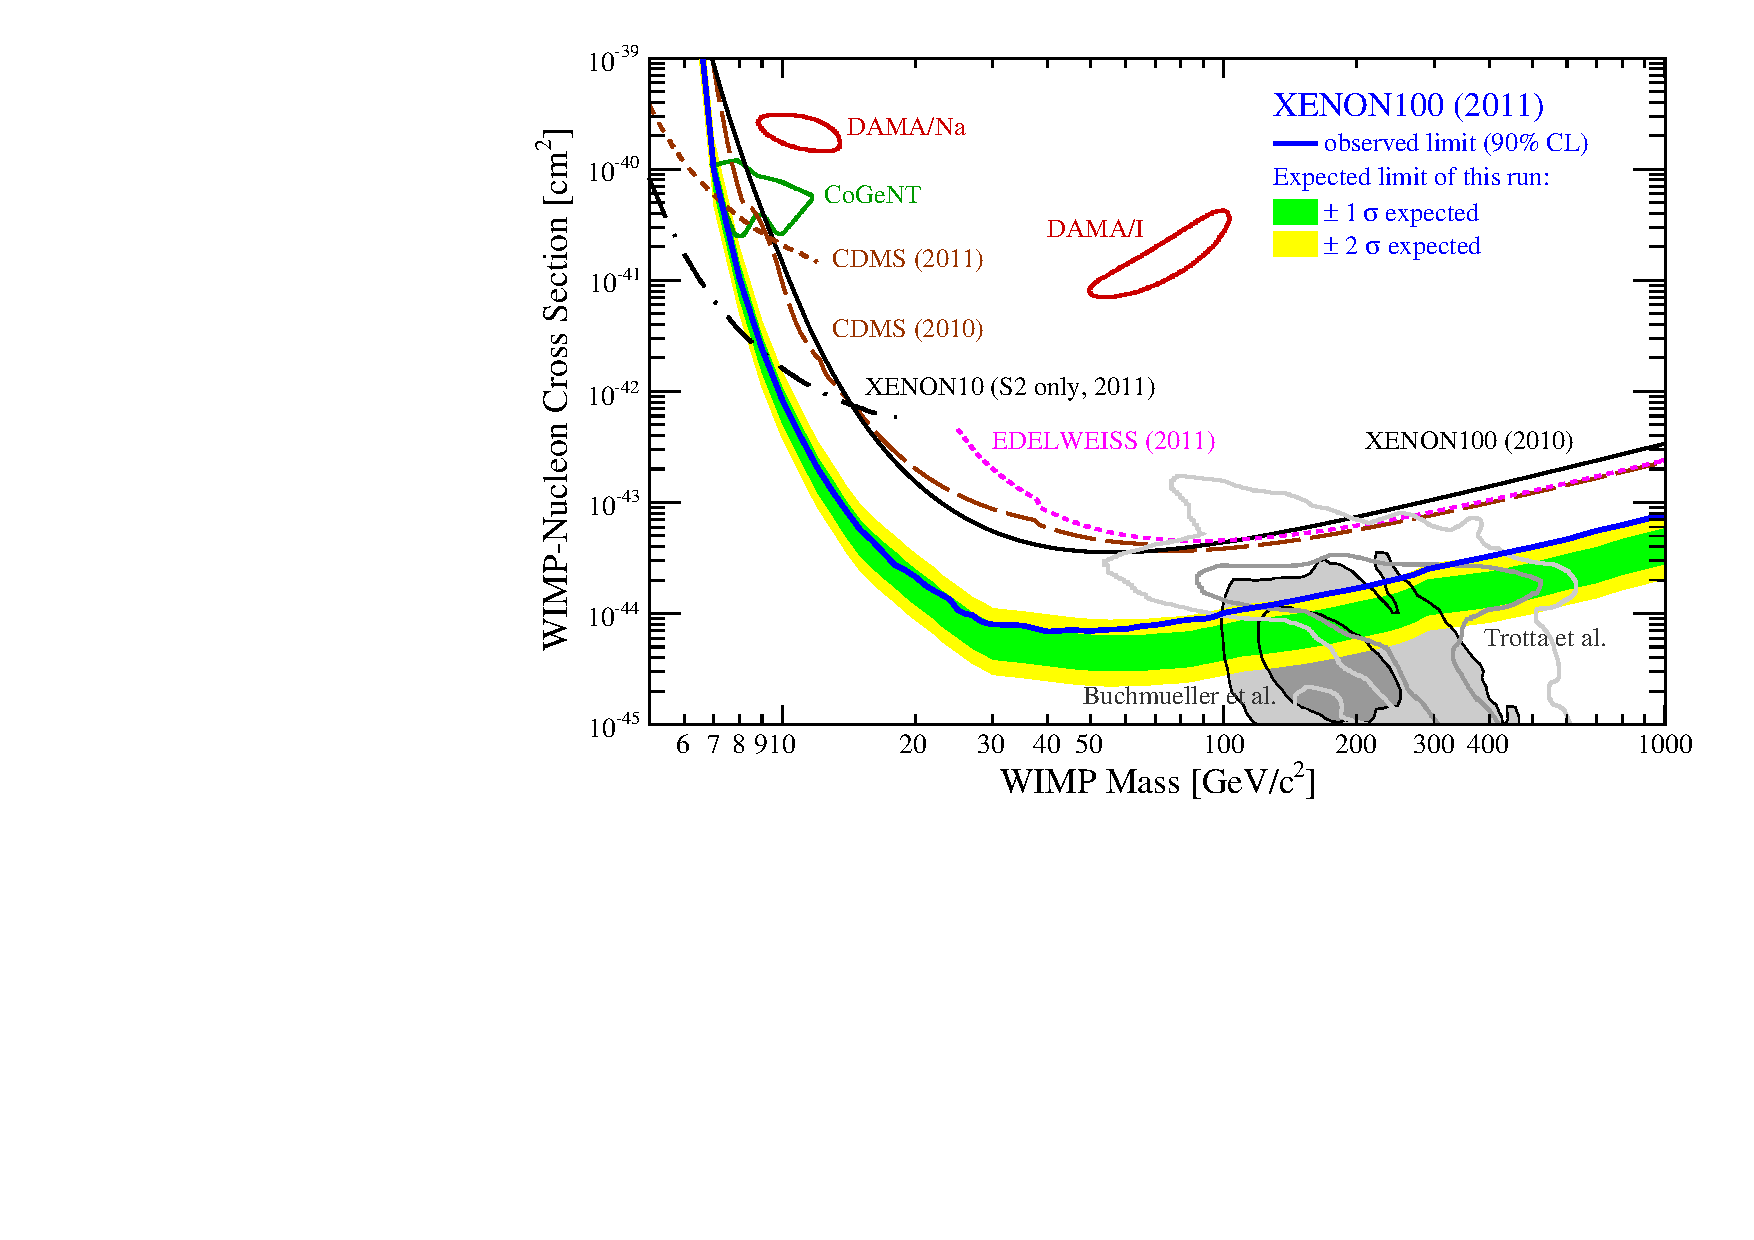
\includegraphics[width=0.9\linewidth]{xenonrun8_limit2}}
\only<10>{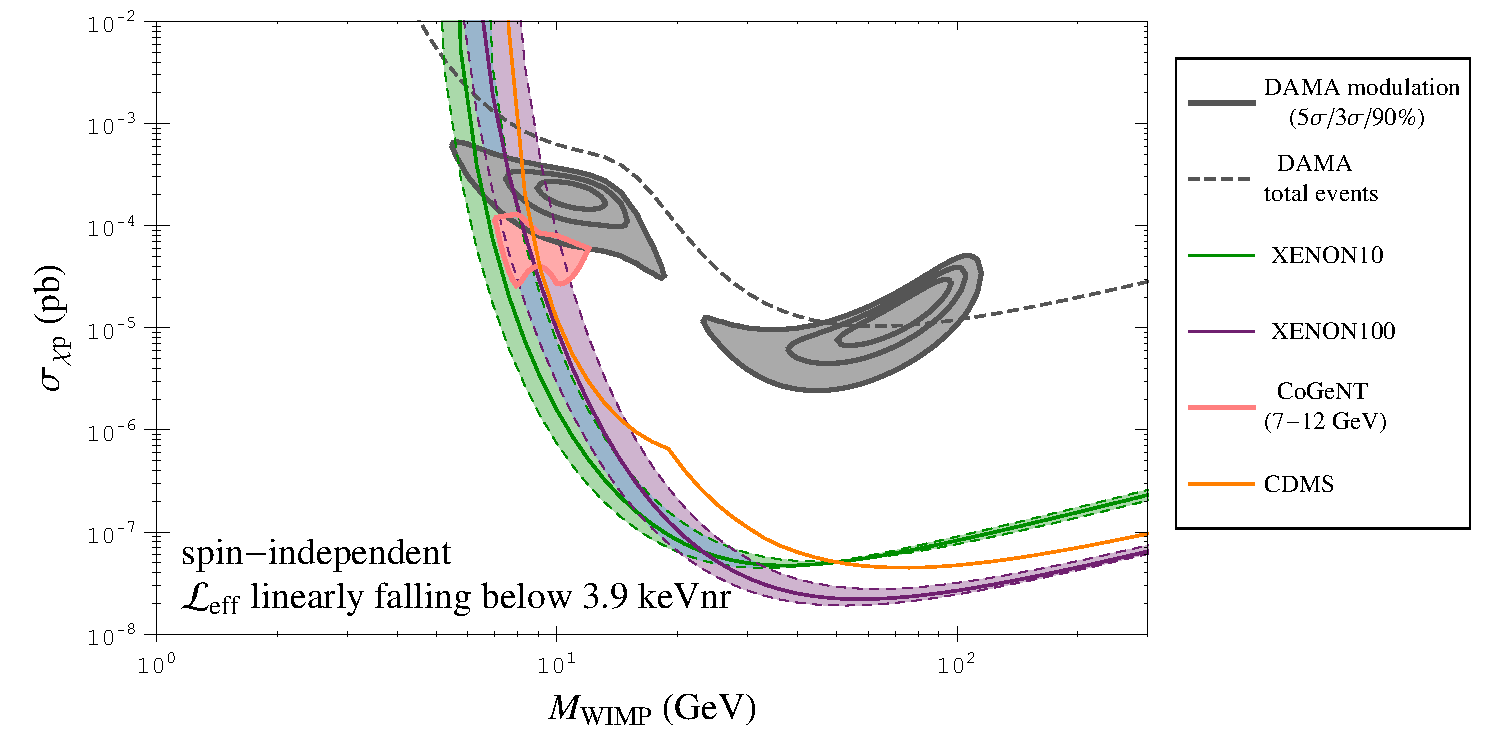
\includegraphics[width=0.9\linewidth]{XENON_falling}}
\end{textblock}

\begin{textblock}{40}(79,50)
\centering
\only<1>{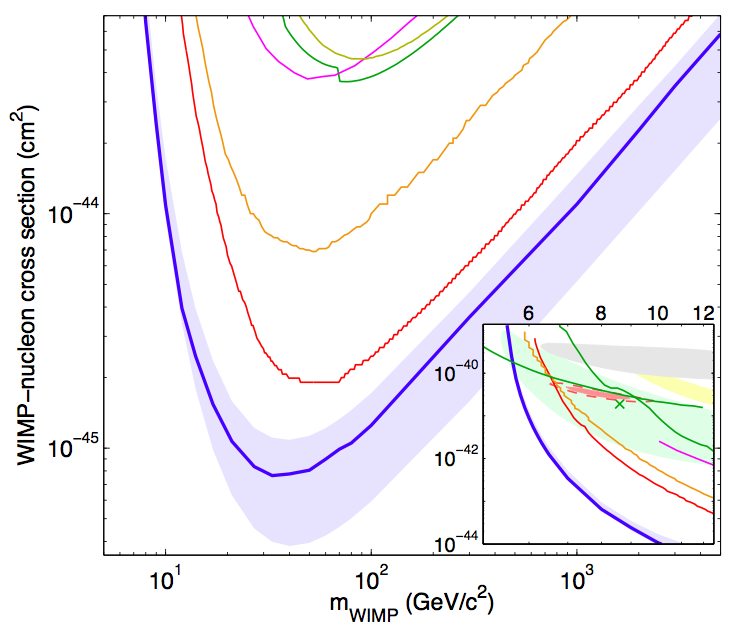
\includegraphics[width=\linewidth]{LUX_fig2}}
\end{textblock}

\begin{textblock}{35}(80,10)
\only<1>{\tiny\color[rgb]{1, 1, 1} XENON-100, \textit{Phys.~Rev.~Lett.} 2011\\LUX, \textit{Phys.~Rev.~Lett.} 2014}\tiny\color[rgb]{0, 0, 0}
\end{textblock}

\begin{textblock}{35}(80,70)
\only<10>{\tiny Savage, Gelmini, Gondolo, Freese \textit{Phys.~Rev.~D} 2011}
\end{textblock}

\visible<2->{Issues:}
\begin{itemize}
\visible<3-9,11>{\item DAMA-LIBRA sees annual modulation of \textit{something} at $8\sigma$}
\visible<4-9,11>{\item CoGeNT has an excess of events at low E, which modulate -- but has issues with surface contamination}
\visible<5-9,11>{\item CRESST-II also has an excess at low E}
\visible<6-9,11>{\item All hints are in low-E regime, where BG modelling is very important, but extremely difficult}
\visible<7-9,11>{\item None of these signals/hints agree}
\visible<8-9,11>{\item All are `excluded' by null results from other experiments}
\visible<9,11>{\item Wiggle-room exists in models, form factors, WIMP halo velocities and detector responses/BGs} 
\visible<11>{\alert{\item $\rightarrow$ exciting, but tricky}}
\end{itemize}

\end{frame}


\begin{frame}

\frametitle{Hitting the ton scale}

Future experiments should shed much more light on the situation

\begin{columns}[t]
\column{0.5\linewidth}
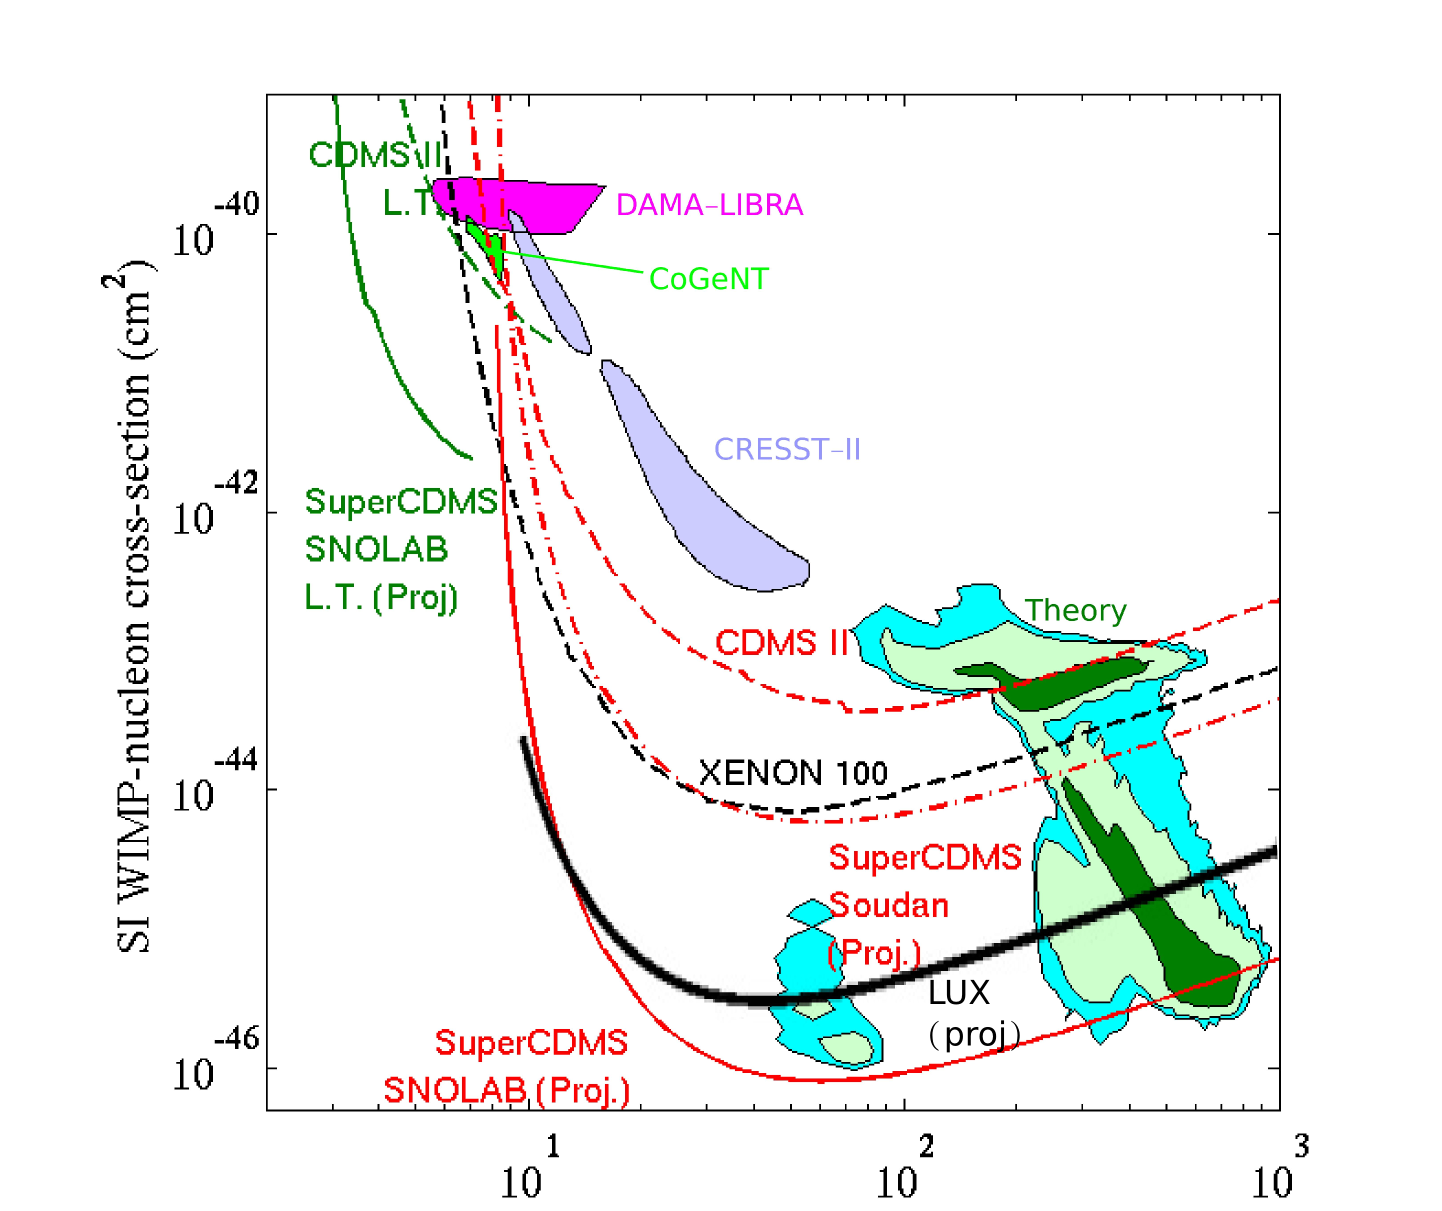
\includegraphics[width=\columnwidth]{dd_proj}\\
XENON-1T, LZ (LUX/ZEPLIN) and SuperCDMS will cover vast areas of parameter space
\column{0.5\linewidth}
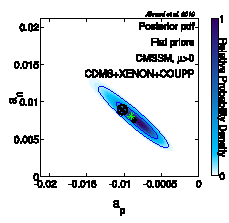
\includegraphics[width=0.9\columnwidth]{Akrami_BM1}

\vspace{4mm}
\centering
{\tiny Akrami, Savage, PS et al, \emph{JCAP} 2010}
\end{columns}

\end{frame}


\subsection[Impacts of dark matter on stars]{Impacts of dark matter on stars \bf(optional)}

  \begin{frame}
    \frametitle{Outline of Lecture 2}
  \begin{columns}[t]
	\column{0.8\textwidth}
	\tableofcontents[sections={1},currentsection,currentsubsection]
        \vspace{3mm}
	\tableofcontents[sections={2},currentsection,currentsubsection]
        \vspace{3mm}
	\tableofcontents[sections={3},currentsection,currentsubsection]
  \end{columns}	
  \end{frame}

\begin{frame}
  \frametitle{Reminder:}

\begin{columns}[c]
\column{0.75\textwidth}
The cartoon version: \begin{enumerate}
\item {Halo WIMPs crash into }\only<1>{the Sun}\only<2->{\cancel{the Sun} \alert<2->{stars}}
\item {Some lose enough energy in the scatter to be gravitationally bound}
\item {Scatter some more, sink to the core}
\item {Annihilate with each other, producing neutrinos \only<3->{\alert{$+$ other energetic particles}}}
\visible<1,4,5>{\item \only<1-3>{Propagate+oscillate their way to the Earth, convert into muons in ice/water}\only<4->{\alert{Particles dump their energy in the stellar core}}}
\visible<1,5>{\item \only<1-4>{Look for \v{C}erenkov radiation from the muons in \textbf{IceCube}, ANTARES, etc}\only<5->{\alert{Stellar structure responds, star evolves accordingly}}}
\end{enumerate}
\column{0.35\textwidth}
  {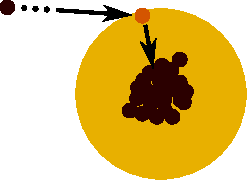
\includegraphics[width=0.8\columnwidth]{comic3_1}}\\
  {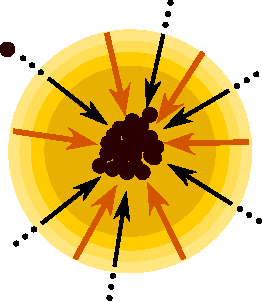
\includegraphics[width=0.6\columnwidth]{comic3_2}}\\
  {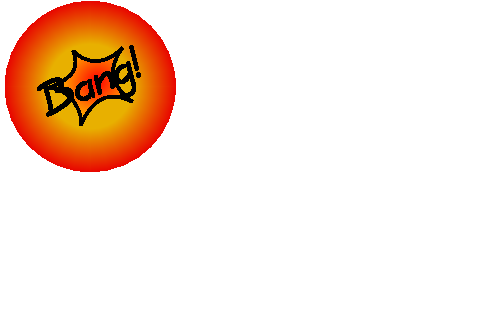
\includegraphics[width=0.6\columnwidth, trim = 0 70 150 0, clip=true]{comic_4}}
\end{columns}

\end{frame}


\begin{frame}
\frametitle{Stellar evolution with dark matter annihilation}
  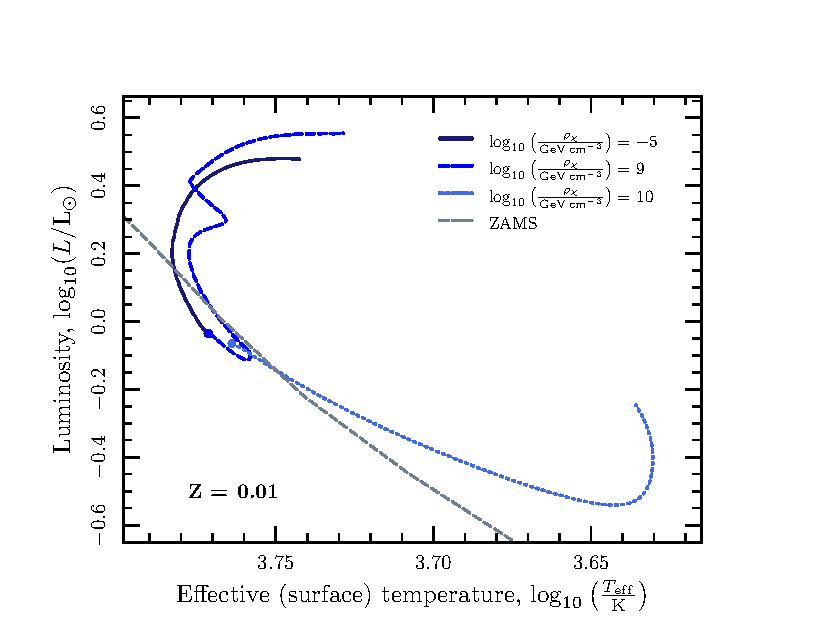
\includegraphics[width=\linewidth, trim = 0 0 0 25, clip=true]{ScottFig1}
\end{frame}


\begin{frame}
  \frametitle{Finding `dark stars'}
  
  \begin{itemize}
    \item
    \uncover<1->{Finding dark stars near the Galactic Centre seems quite possible - not S stars, but low-mass counterparts}
    \item
    \uncover<1->{Best candidates have low masses, elliptical orbits}
    \item
    \uncover<1->{VLT/ELT/TMT/GMT observations should reach the required sensitivity in next few yrs}
    \item
    \uncover<1->{\textsc{DarkStars} stellar evolution code publicly available from {\color[rgb]{0.1, 0.0, 0.6}\href{http://www.fysik.su.se/~pat/darkstars}{\tt http://www.fysik.su.se/{\urltilda}pat/darkstars}}}
  \end{itemize}

  \vfill
  \tiny{\color[rgb]{0, 0, 0} PS, Fairbairn, Edsj\"o, \emph{MNRAS} 2009}\\
  \tiny{\color[rgb]{0, 0, 0} Fairbairn, PS, Edsj\"o, \emph{Phys.~Rev.~D} 2008}
 
\end{frame}

\begin{frame}

  \frametitle{Finding `dark stars'}

  \begin{itemize}
  \item First stars also good targets
  \item Collapsing gas steepens the potential, draws in dark matter
  \item Heating from annihilation can overcome gas cooling and delay collapse
  \item Maybe visible with JWST (if lensed), or by impacts on reionisation
  \end{itemize}\vspace{-3mm}

  {\centering
  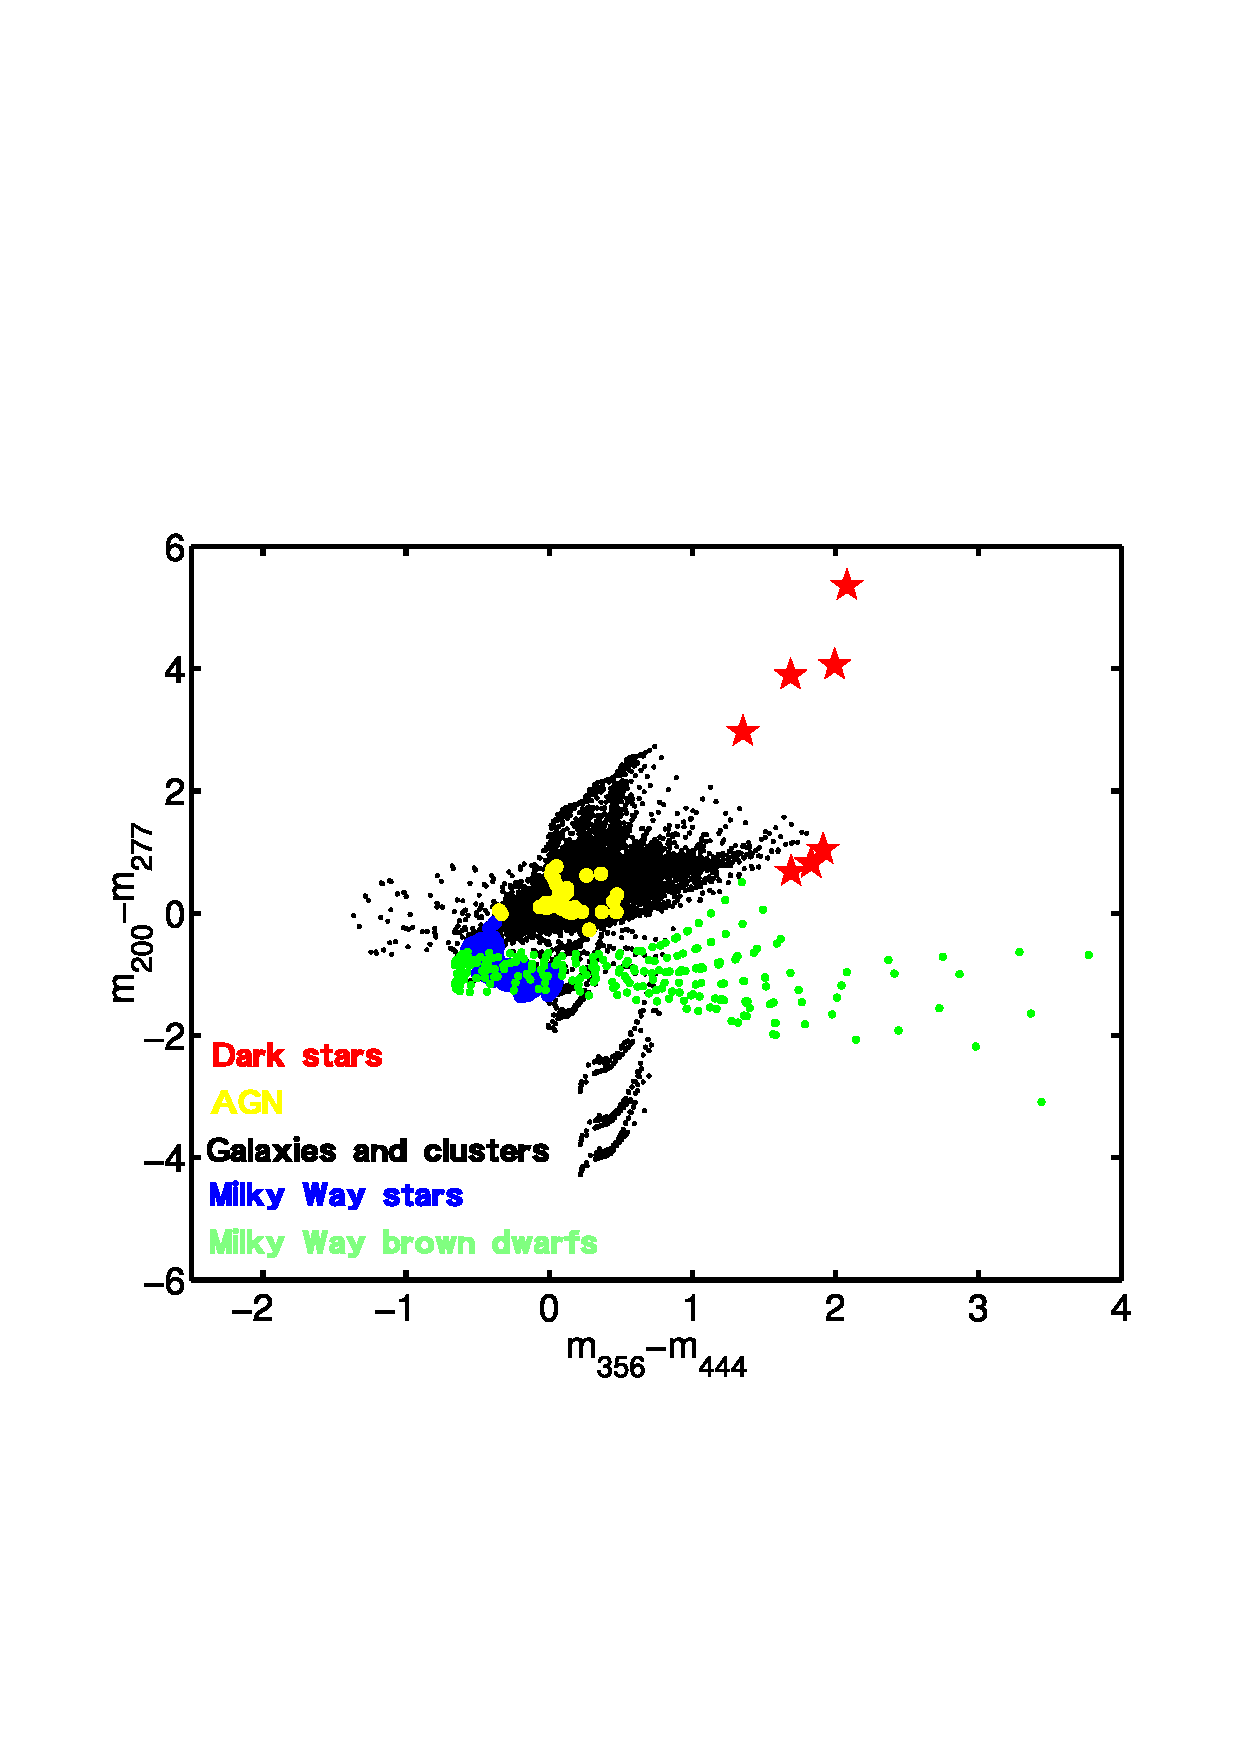
\includegraphics[width=0.33\linewidth, trim = 20 160 20 160, clip=true]{f5_mod}
  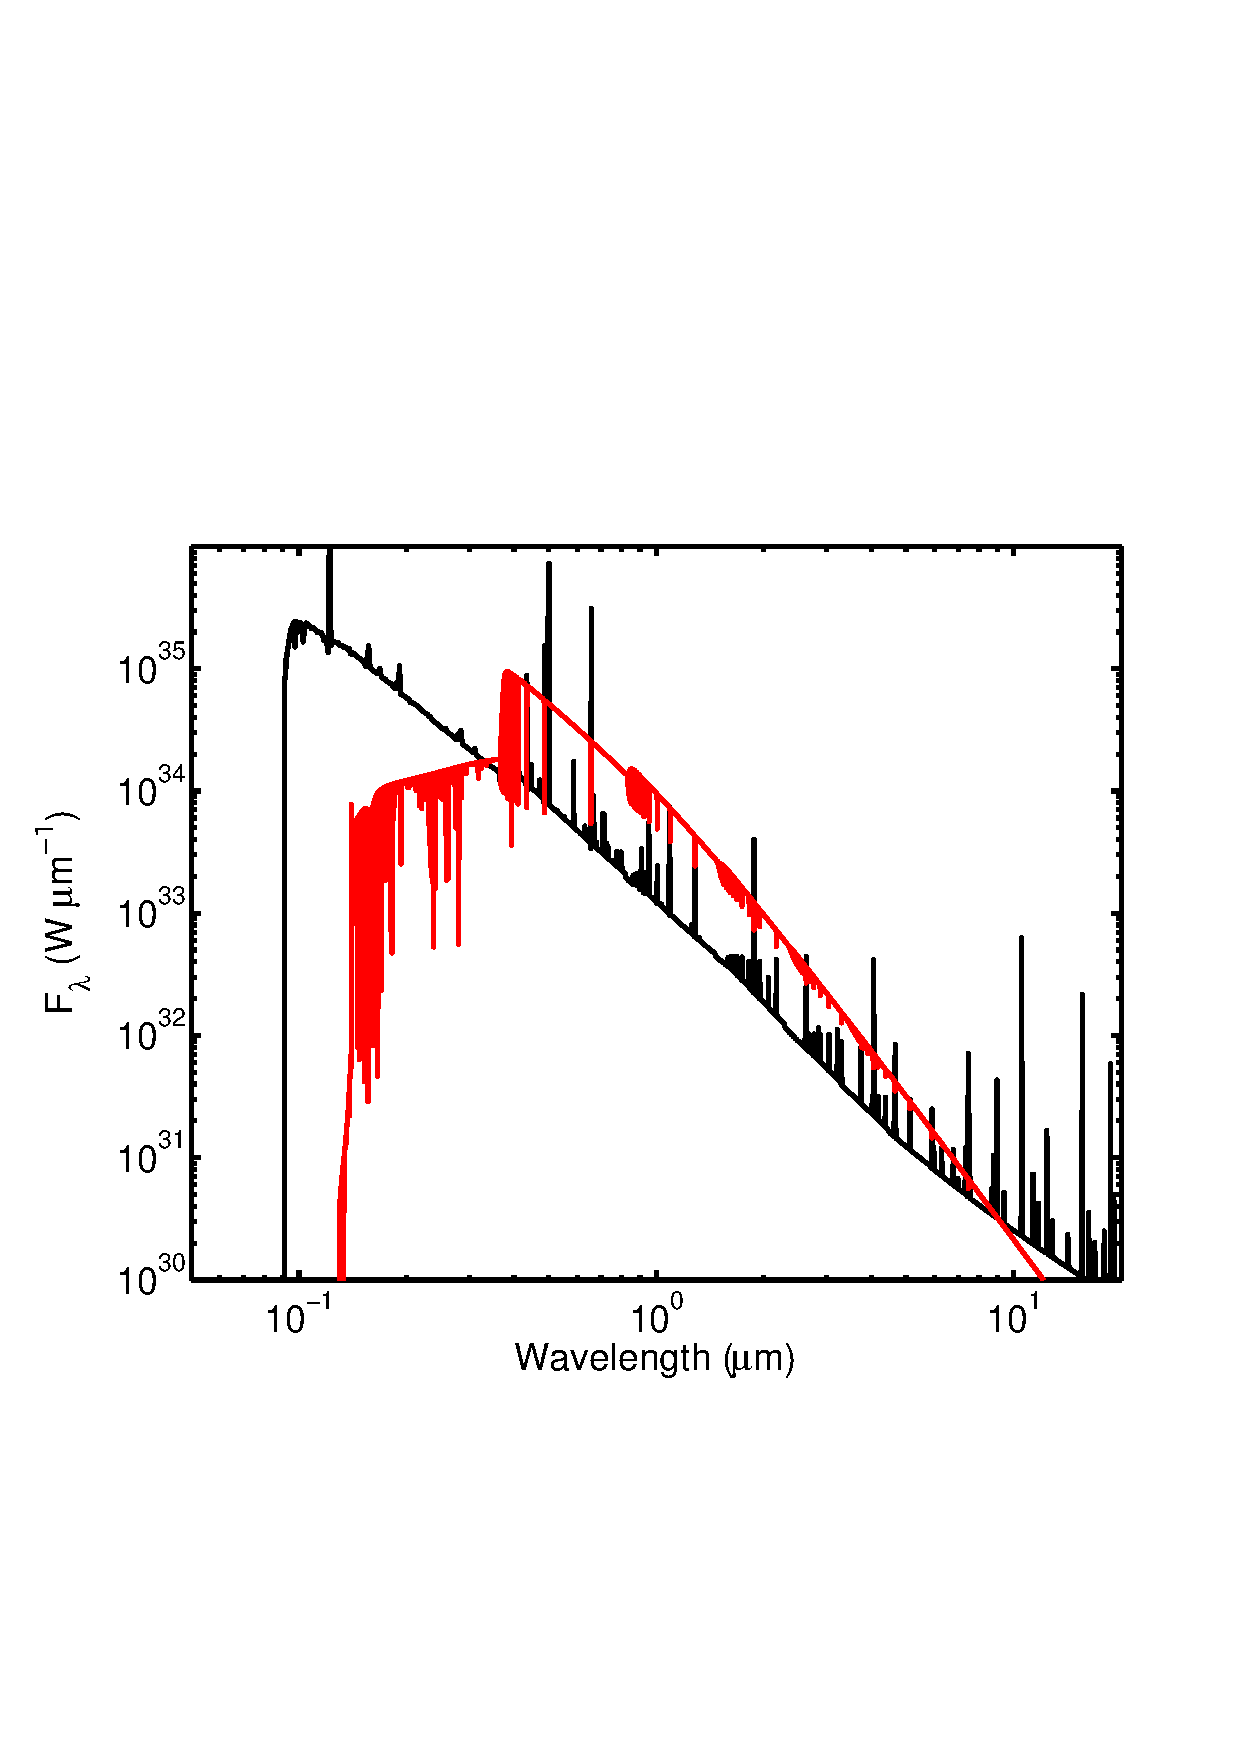
\includegraphics[width=0.33\linewidth, trim = 20 160 20 160, clip=true]{f6}
  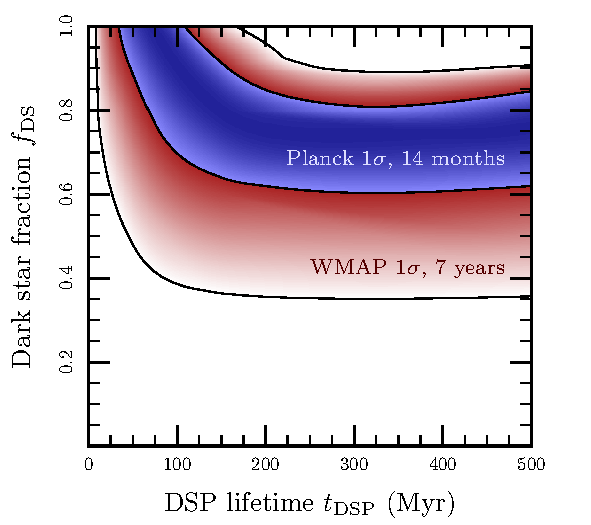
\includegraphics[width=0.33\linewidth]{contour_bounds}
  }

  \tiny{\color[rgb]{0, 0, 0}PS, Venkatesan, Roebber et al \emph{ApJ} 2011}\\
  \tiny{\color[rgb]{0, 0, 0}Zackrisson, PS, Rydberg et al \emph{ApJ} 2010; \emph{MNRAS Lett.} 2010}\\
  \tiny{\color[rgb]{0, 0, 0}Spolyar, Freese, Gondolo, \emph{Phys.~Rev.~Lett.} 2008; Iocco et al, \emph{MNRAS} 2008}

\end{frame}


\begin{frame}
\frametitle{Solar abundances and dark matter}
  
  \begin{itemize}

  \item{New solar composition is 33\% lower in metals than 20 years ago
    \begin{itemize}
    \item{New composition uses state-of-the-art 3D hydro code, improved radiative transfer, non-LTE line formation, best observations, best atomic data, \emph{very} careful line selection}
    \item{Kills agreement with helioseismology \frownie}
    \end{itemize}}

  \visible<1>{\item Something is missing!!  Opacities wrong, weird accretion history (related to planets??), gravity waves, 3D effects or similar missing in interior code\ldots or new physics?}

  \end{itemize}

  \begin{textblock}{55}(60,43)
  \visible<2>{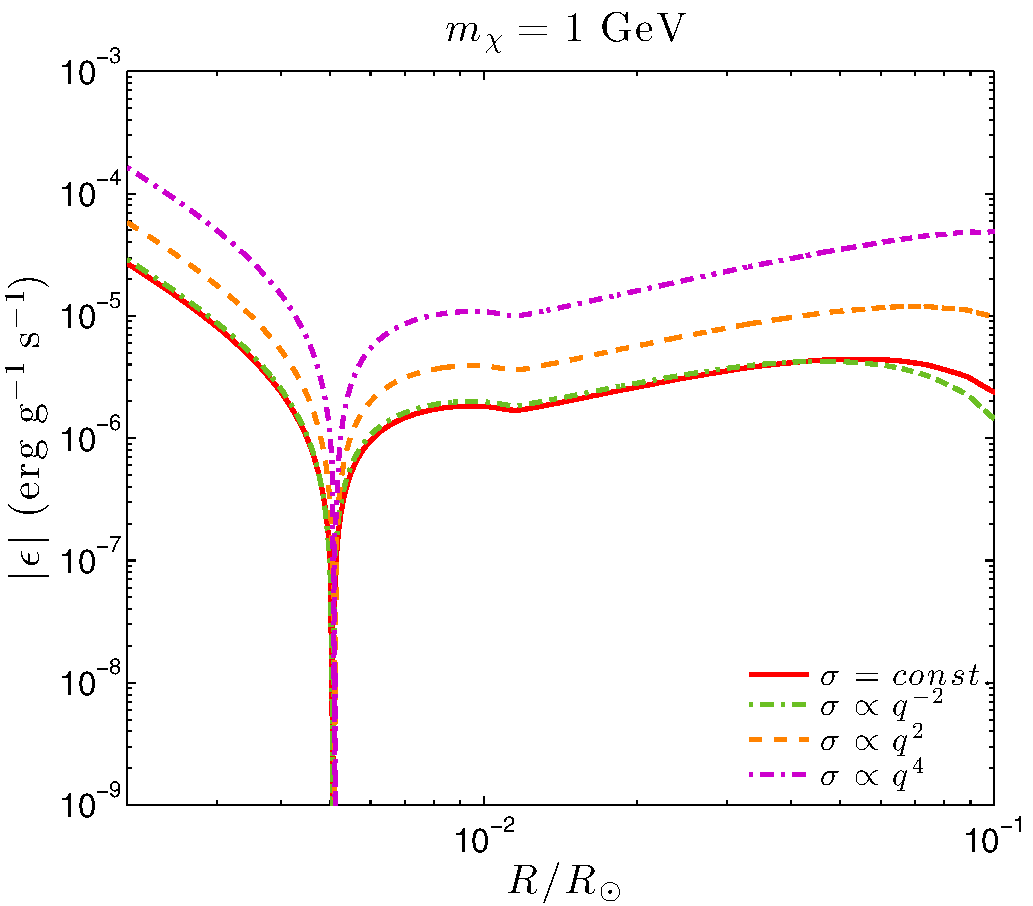
\includegraphics[width=0.85\linewidth]{epsilon_q_m_1}}
  \end{textblock}

  \begin{textblock}{40}(15,50)
  \visible<2>{\color[rgb]{0, 0, 0}Possible solution from momentum-dependent DM?}
  \end{textblock}

  \vspace{20mm}

  \tiny{\color[rgb]{0, 0, 0}\alert<2>{Vincent, PS, \emph{JCAP} in press}}\\
  \tiny{\color[rgb]{0, 0, 0}Serenelli, Basu, Ferguson, Asplund, \emph{ApJL} 2009}\\
  \tiny{\color[rgb]{0, 0, 0}Asplund, Grevesse, Sauval, PS, \emph{Ann Rev A\&A} 2009}

\end{frame}


\begin{frame}
  \frametitle{Summary}

  \begin{itemize}

  \uncover<1->{\item The identity of dark matter can be probed in many complementary ways}

  \uncover<2->{\item Dark matter production in the early Universe places strong constraints on its identity}

  \uncover<3->{\item Indirect detection generally probes masses and annihilation channels}

  \uncover<4->{\item Direct detection probes masses and interactions with quarks}

  \uncover<5->{\item Different probes can (and should) be put together into global fits to gain a consistent picture -- tomorrow.}

  \end{itemize}

\end{frame}


\end{document}

